% !TEX program = xelatex
\documentclass{trinhbay}
\usepackage{xcolor}
\begin{document}

\renewcommand{\bibsection}{%                                             
 \chapter*{\bibname}}
 
%!TEX root = ../luanvan.tex
\begin{titlepage}
        \parindent0pt

        \pagestyle{empty}

        \begin{center}
                \textbf{\large \textsc{BỘ GIÁO DỤC VÀ ĐÀO TẠO \\TRƯỜNG ĐẠI HỌC CẦN THƠ}}
                \vspace{30mm}
                \\
                \textbf{\large DƯƠNG TUẤN DŨNG}
                \vspace{35mm}
                \\
                \textbf{\huge XÂY DỰNG HỆ THỐNG QUẢN LÝ VĂN BẰNG CHỨNG CHỈ SỬ DỤNG CÔNG NGHỆ BLOCKCHAIN}
                \vspace{45mm}
                \\
                \textbf{\large LUẬN VĂN THẠC SĨ \\ NGÀNH KHOA HỌC MÁY TÍNH  \\ MÃ SỐ 8480101}
                \vspace{60mm}
                \\
                \textbf {\large NĂM 2022}
        \end{center}

        \clearpage
        \begin{center}
                \textbf{\large \textsc{BỘ GIÁO DỤC VÀ ĐÀO TẠO \\TRƯỜNG ĐẠI HỌC CẦN THƠ}}
                \vspace{30mm}
                \\
                \textbf{\large DƯƠNG TUẤN DŨNG}
                \\
                \textbf{\large{MÃ SỐ HV: M3718005}}
                \vspace{35mm}
                \\
                \textbf{\huge XÂY DỰNG HỆ THỐNG QUẢN LÝ VĂN BẰNG CHỨNG CHỈ SỬ DỤNG CÔNG NGHỆ BLOCKCHAIN}
                \vspace{45mm}
                \\
                \textbf{\large LUẬN VĂN THẠC SĨ \\ NGÀNH KHOA HỌC MÁY TÍNH  \\ MÃ SỐ 8480101}
                \\
		\vspace{20mm}
		
                \textbf{\large{NGƯỜI HƯỚNG DẪN} }
		\\
		\textbf{\large{TS. NGUYỄN VĂN HÒA} }
		\\
		\vspace{30mm}
                
                \textbf {\large NĂM 2022}
        \end{center}
\end{titlepage}
\setstretch{1.2}
\pagenumbering{roman}
%%!TEX root = ../luanvan.tex
\chapter*{Trang xác nhận của hội đồng}
Xác nhận của hội đồng
%!TEX root = ../luanvan.tex
\chapter*{Lời cảm ơn}
Để hoàn thành luận văn này, tôi xin gửi lời cảm ơn chân thành đến:

Thầy hướng dẫn TS. Nguyễn Văn Hòa, thầy đã đồng hành và hướng dẫn tôi trong quá trình học tập cũng như trong việc hoàn thành luận văn.

Thầy, cô Khoa Công nghệ Thông tin và Truyền thông Trường Đại học Cần Thơ đã tận tình giảng dạy cho tôi trong thời gian học tập.

Xin cảm ơn Ban Giám hiệu Trường Đại học An Giang, Ban Giám đốc Trung tâm Tin học Trường Đại học An Giang đã tạo điều kiện thuận lợi trong suốt thời gian đi học và làm bài luận văn.

Xin cảm ơn đến gia đình, thầy, cô, anh, chị đồng nghiệp, bạn bè và anh chị học viên lớp KHMT-K25, những người đã luôn sẵn sàng chia sẻ và hỗ trợ nhau trong học tập và trong cuộc sống.

Do giới hạn kiến thức và khả năng của bản thân còn nhiều thiếu sót và hạn chế, kính mong sự chỉ dẫn và đóng góp của thầy, cô để bài luận văn của tôi được hoàn thiện hơn.
\begin{center}
\begin{longtable}{cc}

\hspace{40mm} & \textit{Cần Thơ, ngày \ldots{} tháng \ldots{}  năm 2022 } \\ 
 & \textbf{Học viên} \\ 
\\
\\

 & \textbf{Dương Tuấn Dũng}  \\ 

\end{longtable}
\end{center}
%!TEX root = ../luanvan.tex
\chapter*{Tóm tắt}
\addcontentsline{toc}{chapter}{Tóm tắt}
Ứng dụng công nghệ thông tin vào quản lý văn bằng, chứng chỉ đã giúp tăng đáng kể hiệu quả công tác. Phần mềm quản lý giúp đơn vị quản lý, người có văn bằng, chứng chỉ trong việc tra cứu; các tổ chức có liên quan xác minh, công nhận văn bằng, chứng chỉ. Đồng thời thông tin cấp văn bằng, chứng chỉ được công khai, bảo đảm tính bảo mật thông tin cá nhân của người được cấp văn bằng, chứng chỉ. 

Với mục đích đảm bảo tính an toàn, bảo mật thông tin và giải quyết vấn đề tồn tại khi đối chiếu thông tin thủ công, đề tài nghiên cứu xây dựng hệ thống quản lý văn bằng chứng chỉ sử dụng công nghệ blockchain. Mạng blockchain Hyperledger Fabric được dùng để triển khai mô hình thử nghiệm lưu trữ thông tin văn bằng chứng chỉ lên chuỗi khối sau đó với tùy chọn chia sẻ thông tin cá nhân của người xác minh với bên cần xác minh.

Hệ thống thử nghiệm trong đề tài thực hiện quá trình xác thực quyền truy cập thông qua máy chủ. Thông tin văn bằng chứng chỉ có thể được xác thực và tin cậy nhờ chữ ký số nội bộ của Hyperledger Fabric. Giao diện thử nghiệm được phát triển trên nền tảng web để người dùng có thể dễ dàng sử dụng. Dựa trên kết quả thử nghiệm, hệ thống quản lý đáp ứng được yêu cầu kỹ thuật bao gồm: cấp phát chứng chỉ, xác minh chứng chỉ hợp lệ với tùy chọn hạn chế lộ thông tin cá nhân.

%!TEX root = ../luanvan.tex
\chapter*{Abstract}
\addcontentsline{toc}{chapter}{Abstract}
Applying information technology to the management of diplomas and certificates has increased significantly in overall efficiency. The information management system helps the issuers, verifiers, the owners of diplomas and certificates in issuing, searching, verifying, and recognizing diplomas and certificates. At the same time, it ensures the confidentiality of the personal information of the diploma or certificate holders which is made public.

To ensure the privacy and confidentiality of the information and solve problems that exist when comparing information by hand, the research topic is the certificate management system based on blockchain technology. A Hyperledger Fabric blockchain network is used to deploy a proof of concept model that stores certificate information on the blockchain and then verifies it with specific disclosure of the owner’s information to the party that needs to verify.

In the model, the authentication of access rights is performed through a server. Thanks to Hyperledger Fabric's internal digital signatures, certificate information can be authenticated and trusted. The model’s interface is developed using a web platform so that users can easily use it. Based on the test results, the certificate management system meets the technical requirements including issuing certificates and verifying valid certificates through less personal information disclosure.

%!TEX root = ../luanvan.tex
\chapter*{Lời cam đoan}
Tôi tên là Dương Tuấn Dũng, là học viên ngành Khoa học máy tính, khóa 2018-2020. Tôi xin cam đoan luận văn này là công trình nghiên cứu khoa học thực sự của bản thân tôi được sự hướng dẫn của TS. Nguyễn Văn Hòa.

Các thông tin được sử dụng tham khảo trong đề tài luận văn được thu thập từ các nguồn đáng tin cậy, đã được kiểm chứng, được công bố rộng rãi và được tôi trích dẫn nguồn gốc rõ ràng ở phần Danh mục Tài liệu tham khảo. Các kết quả nghiên cứu được trình bày trong luận văn này là  do chính tôi thực hiện một cách nghiêm túc, trung thực và không trùng lắp với các đề tài khác đã được công bố trước đây.

Tôi xin lấy danh dự và uy tín của bản thân để đảm bảo cho lời cam đoan này.

\begin{table}[h]
  \begin{tabular}{ p{7cm}  p{8cm} }
                                   & \emph{Cần Thơ, ngày \ldots{ } tháng \ldots{ } năm 2022}\\
\hspace{20mm}\textbf{Người hướng dẫn}& \hspace{22mm}\textbf{Tác giả thực hiện}\\
									& \\
									& \\
									& \\
         & \\

\hspace{1.6cm}\textbf{TS. Nguyễn Văn Hòa}	&\hspace{2.1cm}\textbf{Dương Tuấn Dũng}\\
                                    
\end{tabular}
\end{table}

\setstretch{1}
\tableofcontents
\addcontentsline{toc}{chapter}{\contentsname}
\listoftables
\listoffigures
%!TEX root = ../luanvan.tex
\chapter*{Danh mục từ viết tắt}
\begin{center}
\renewcommand{\arraystretch}{1.5}
\begin{longtable}{ |l @{\qquad} |l| }
\hline
CSDL   & Cơ sở dữ liệu  \\ \hline
LTS  &  Long Term Support  \\ \hline
PKI  &  Public Key Infrastructure \\ \hline
API    & Application Programming Interface  \\ \hline
CA    & Certificate Authority \\ \hline
SDK    & Software Development Kit \\ \hline

\end{longtable}
\end{center}

\setstretch{1.2}
\pagenumbering{arabic}

%!TEX root = ../luanvan.tex
\chapter{Mở đầu}

\section{Giới thiệu}

Đề tài nghiên cứu xây dựng hệ thống quản lý văn bằng, chứng chỉ sử dụng công nghệ blockchain.
Ngày nay, các hệ thống ứng dụng công nghệ thông tin có vai trò ngày càng quan trọng.
Trong lĩnh vực giáo dục, những hệ thống này giúp thu thập, quản lý thông tin, tạo ra các sản phẩm thông tin phục vụ nhu cầu học tập, giảng dạy và quản lý.
Một trong những sản phẩm thông tin đó là văn bằng, chứng chỉ (VBCC).
Điều 26 của Quy chế ban hành theo Thông tư số 21/2019/TT-BGDĐT  có quy định công bố công khai thông tin về cấp VBCC trên cổng thông tin điện tử.
Ngoài ra, VBCC là một chứng cứ học tập của người sở hữu và có vai trò cần thiết trong nghề nghiệp.
Cá nhân được đào tạo và nhận chứng nhận trước khi có thể bắt đầu công việc của mình.
Do đó, thông tin dữ liệu về VBCC cần được quan tâm, bảo đảm lưu trữ an toàn, tin cậy và sẵn sàng.

Công nghệ blockchain hay công nghệ chuỗi khối có những đặc tính rất hữu ích trong việc lưu trữ, xử lý và chuyển giao thông tin một cách an toàn, tin cậy có thể đáp ứng các điều kiện về an toàn thông tin.
Công nghệ chuỗi khối là công nghệ mã hóa và lưu trữ thông tin thành các khối và liên kết lại với nhau.
Mỗi khi thông tin hoặc giao dịch mới xảy ra, thông tin cũ sẽ không bị mất đi mà thay vào đó, thông tin mới sẽ được lưu vào một khối mới và lần lượt được nối vào khối cũ để tạo thành chuỗi.
Hơn nữa, dữ liệu của chuỗi khối được lưu trữ phân tán trên các máy chủ kết nối trong hệ thống blockchain để mọi người có thể xem và xác minh các giao dịch. Điều này có thể ngăn chặn việc sửa đổi hoặc gian lận và đảm bảo tính minh bạch và an toàn thông tin.

Trong đề tài, công nghệ blockchain được ứng dụng vào quản lý VBCC trong việc lưu trữ thông tin VBCC trên chuỗi khối để đảm bảo thông tin an toàn, tin cậy, minh bạch và bền vững theo thời gian.
Ngày nay, VBCC chủ yếu được quản lý dưới dạng hồ sơ giấy và việc cấp VBCC chưa được số hóa.
Hồ sơ giấy được xem là dữ liệu gốc bao gồm các VBCC được in lên mẫu phôi và những hồ sơ theo quy định. Hồ sơ gốc có chữ ký tay và được đóng dấu của đơn vị cấp VBCC theo quy định tại Điều 20 của Thông tư số 21/2019/TT-BGDĐT.
Ứng dụng của blockchain để số hóa việc cấp VBCC và xác thực thông tin VBCC được khảo sát trên một số công nghệ blockchain khá phổ biến hiện nay như Hyperledger Fabric, Ethereum, BigchainDB.
Trong những công nghệ blockchain này, ứng dụng của hợp đồng thông minh trên nền tảng Hyperledger Fabric sẽ thực hiện số hóa việc cấp VBCC, thông tin của VBCC được mã hóa và lưu trữ vào chuỗi khối.

Công nghệ blockchain là một xu hướng công nghệ ngày nay và được ứng dụng trong nhiều ngành, lĩnh vực khác nhau. Một số công trình nghiên cứu liên quan công nghệ blockchain như sau.

Trong lĩnh vực an toàn thông tin có các ứng dụng giúp dữ liệu trên blockchain được toàn vẹn, chống làm giả. Nghiên cứu \cite{ralphcharlesmerkle1979} của Ralphe Charles Merkle về ứng dụng hệ mật mã khóa công khai trong an toàn thông tin.
Với các hệ mật mã chỉ dùng một khóa duy nhất trong mật mã và giải mật, khóa này được tạo ra và được mỗi bên giữ bí mật để bảo mật thông tin. 
Tuy nhiên, vấn đề trao đổi khóa gặp nhiều khó khăn trong thực tiễn.
Ngoài ra, với một khóa duy nhất thì vai trò mỗi bên như nhau trong liên lạc.
Với các hệ mật mã khóa công khai, mỗi bên tạo một cặp khóa.
Trong đó, một khóa công bố công khai cho tất cả và một khóa riêng tư được mỗi bên giữ bí mật.
Khóa công khai chỉ liên kết với khóa riêng tư, đảm bảo rất khó để người khác tạo ra khóa công khai mà không biết khóa cá nhân tương ứng.
Bài giảng \cite{lequyetthang2016} có giải thích rằng các giải pháp mật mã với khóa công khai ra đời nhằm cá nhân hóa mật mã.
Đó là các giải pháp Diffie-Helmann, ElGamma và RSA (viết tắt tên của 3 sinh viên trường Stanford: Rivest, Shamir và Adleman).
Các giải pháp này vẫn còn nguyên giá trị đến ngày nay.
Chữ ký số ra đời sau đó và được phát triển cùng với các giải pháp Băm (Hash) kết hợp với mật mã khóa công khai. 

Trong lĩnh vực y tế và chăm sóc sức khỏe, nghiên cứu \cite{ANTWI2021100012} đề xuất giải pháp ứng dụng công nghệ blockchain riêng tư trong quản lý và bảo vệ quyền sở hữu thông tin sức khỏe của bệnh nhân.
Những thông tin này quan trọng đối với người bệnh, nhà thuốc, công ty bảo hiểm và nhà nghiên cứu.
Do đó, thông tin này cần được quan tâm tránh rò rỉ khi chia sẻ thông tin người bệnh.
Nghiên cứu chỉ ra rằng Hyperledger Fabric có thể đáp ứng về tính an toàn, dễ mở rộng, tuân thủ luật pháp và linh hoạt trong quản lý thông tin sức khỏe của bệnh nhân.   

Trong lĩnh vực giáo dục ở các nước trên thế giới và Việt Nam đang đẩy mạnh số hóa thông tin đào tạo.
Trong đó công nghệ blockchain được dùng để làm cơ sở dữ liệu bảo mật trong việc lưu trữ thông tin bằng cấp của sinh viên và thông tin quá trình đào tạo.
Công nghệ blockchain giúp tránh tình trạng gian lận trong quá trình học tập của sinh viên.
Phòng nghiên cứu truyền thông thuộc Viện Công nghệ Massachusetts, Hoa Kỳ nghiên cứu dự án Blockcerts để số hóa chứng nhận cho các học viên hoàn thành chương trình MIT trên nền tảng blockchain.
Blockcerts cung cấp tiêu chuẩn mở để tạo, phát hành, xem và xác minh các chứng chỉ dựa trên blockchain.
\section{Lý do chọn đề tài}

Hiện nay, các hồ sơ dữ liệu liên quan VBCC được quản lý lưu trữ tập trung tại đơn vị cấp VBCC.
Sinh viên nhận được VBCC dưới dạng bản in.
Tuy nhiên, khi có yêu cầu xác thực thông tin VBCC, phải thông qua đơn vị quản lý VBCC tra cứu hồ sơ và thường tốn nhiều thời gian.
Vì vậy, công nghệ blockchain có thể giải quyết vấn đề liên quan đến tra cứu, xác minh, công nhận VBCC. Thông tin VBCC được lưu trên blockchain có đặc tính chống sửa đổi và đảm bảo tính toàn vẹn dữ liệu.  

Trung tâm Tin học Trường Đại học An Giang là đơn vị hoạt động về lĩnh vực đào và có chức năng tổ chức thi và cấp chứng chỉ.
Công tác quản lý về đào tạo, tổ chức thi và cấp chứng chỉ tại đơn vị đã được tin học hóa một số nghiệp vụ mang lại hiệu quả đáng kể như ghi danh học viên, quản lý hóa đơn, nhận hồ sơ dự thi, tra cứu điểm thi, và công khai thông tin VBCC do đơn vị cấp trên hệ thống website.

Sổ gốc cấp VBCC theo quy định tại Điều 19 thông tư số 21/2019/TT-BGDĐT yêu cầu ghi thông tin cấp phát VBCC cho người được cấp, đã thi đạt sau khi dự thi tại cơ sở tổ chức thi. Sổ gốc cấp VBCC phải được ghi chính xác, đánh số trang, đóng dấu giáp lai, không được tẩy xóa, đảm bảo quản lý chặt chẽ và lưu trữ vĩnh viễn. Tuy nhiên, việc cập nhật thông tin thay đổi vào sổ, theo dõi sổ gốc còn làm thủ công trong những trường hợp như sau:

\begin{enumerate}
\item Nhân viên phát VBCC cho người nhận chứng chỉ đến trực tiếp và có giấy tờ khớp thông tin với sổ gốc thì nhân viên phát cho người đó và cập nhật sổ gốc. Ngược lại, nếu giấy tờ người nhận mang theo mà thông tin không khớp với sổ gốc thì nhân viên không phát cho người đó.

\item Nhân viên phát VBCC cho người nhận chứng chỉ có giấy ủy quyền đến trực tiếp và có giấy tờ ủy quyền khớp thông tin với sổ gốc thì nhân viên phát cho người đó và cập nhật sổ gốc. Ngược lại, nếu giấy tờ người nhận mang theo mà thông tin không khớp với sổ gốc thì nhân viên không phát cho người đó.

\item Văn bằng, chứng chỉ chưa phát phải được quản lý, lưu trữ theo quy định.
\end{enumerate}

Mặt khác những trường hợp 1, 2, dù không phát VBCC vẫn phải so khớp thông tin giấy tờ với sổ gốc, nên công việc chưa được hiệu quả. Thêm vào đó, xử lý trên hồ sơ giấy có thể gặp một số rủi ro như rách trang giấy, thất lạc,\ldots{} làm ảnh hưởng đến công tác lưu trữ, bảo quản hồ sơ theo quy định.

Mục tiêu chính của đề tài là ứng dụng công nghệ Blockchain để lưu trữ thông tin VBCC. Ngoài việc tìm hiểu những khái niệm liên quan công nghệ chuỗi khối với các đặc tính công khai, an toàn, minh bạch, đề tài còn hướng đến nhu cầu dùng công nghệ chuỗi khối để kiểm chứng thông tin VBCC khi thông tin được truy vấn từ cơ sở dữ liệu VBCC bên ngoài chuỗi khối.

\section{Mục tiêu nghiên cứu}

Đề tài tập trung đề xuất mô hình ứng dụng công nghệ Blockchain trong quản lý VBCC nhằm hỗ trợ theo dõi việc cập nhật thông tin cho người sử dụng nhưng vẫn đảm bảo tính minh bạch, công khai và an toàn. Các mục tiêu cụ thể như sau:

\begin{enumerate}
\item Phân tích và xây dựng CSDL đáp ứng nghiệp vụ quản lý VBCC: cập nhật thông tin sổ gốc cấp VBCC; tra thông tin VBCC.
\item Xây dựng hệ thống website tương tác với người sử dụng, giao diện trực quan và phản hồi nhanh.
\item Xây dựng mạng Hyperledger Fabric và triển khai lưu trữ dữ liệu nhật ký về VBCC trên mạng này.
\end{enumerate}

\section{Đối tượng và phạm vi nghiên cứu}

Đối tượng nghiên cứu:

\begin{itemize}
\item Lý thuyết mật mã có liên quan công nghệ chuỗi khối
\item Mô hình mạng thử nghiệm Hyperledger Fabric
\item Quy định pháp luật về quản lý VBCC
\end{itemize}

Phạm vi nghiên cứu:

\begin{itemize}
\item Quy trình cấp phát chứng chỉ của Trung tâm Tin học Trường Đại học An Giang
\item Xây dựng hệ thống quản lý VBCC ứng dụng công nghệ blockchain.
\end{itemize}

\section{Phương pháp nghiên cứu}

\begin{itemize}
\item Tìm hiểu, phân tích và tổng hợp tài liệu về quản lý VBCC (quy định, biểu mẫu hiện hành) và các nền tảng kiến trúc, cơ chế hoạt động của mạng Blockchain.
\item Xác định các quy trình nghiệp vụ, yêu cầu của hệ thống, cơ sở dữ liệu, thông tin được lưu trên chuỗi khối.
\item Phương pháp thực nghiệm, ghi nhận kết quả và đánh giá kết quả đạt được.
\end{itemize}
\section{Ý nghĩa của đề tài}

Đề tài có tính ứng dụng cao, bên cạnh việc tìm hiểu kiến thức, những khái niệm liên quan công nghệ chuỗi khối.
Ngoài việc triển khai với bài toán cụ thể tại Trung tâm Tin học Trường Đại học An Giang trong quản lý VBCC, nghiên cứu có thể ứng dụng ở các đơn vị khác có nghiệp vụ tương tự như các trường học, cơ sở đào tạo.

Công nghệ chuỗi khối có khả năng lưu trữ, xử lý và chia sẻ thông tin, dữ liệu minh bạch theo thời gian và có độ an toàn cao. Các nghiên cứu về công nghệ chuỗi khối có thể mở rộng ứng dụng trong nhiều lĩnh vực như nông nghiệp, y tế, ngân hàng, vận tải.
\section{Tiểu kết chương 1}

Chương 1 trình bày các mục tiêu của hệ thống cần đạt được trong quá trình nghiên cứu và thực hiện. Chương 2 sẽ tập trung giới thiệu cơ sở lý thuyết quản lý VBCC, đặc tính an toàn, bảo mật của công nghệ chuỗi khối, và mô hình mạng thử nghiệm Hyperledger Fabric.

%!TEX root = ../luanvan.tex
\chapter{Cơ sở lý thuyết}
\section{Quản lý văn bằng chứng chỉ}
\subsection{Giới thiệu}

Xã hội ngày càng phát triển nên nhu cầu học tập nâng cao trình độ đáp ứng cho các lĩnh vực lao động xã hội ngày càng tăng.
Hàng năm có hàng nghìn các loại văn bằng, chứng chỉ được cấp phát để công nhận trình độ, năng lực của các học viên đã qua một quá trình học tập và thi đạt.
Ngoài ra, văn bằng được dùng trong tuyển dụng lao động và làm thủ tục hồ sơ liên quan khác, ảnh hưởng nhiều đến người sở hữu trong tương lai.
Trong nhiều ngành nghề, chứng chỉ là điều kiện để thực hiện công việc, có tính quyết định và ảnh hưởng tới nhiều lĩnh vực khác.
Do đó, quản lý văn bằng chứng chỉ đòi hỏi quy trình thực hiện nghiêm ngặt, tránh những trường hợp lợi dụng kẽ hở để thực hiện hành vi trái pháp luật.

Một số văn bản pháp luật được ban hành nhằm quy định việc quản lý văn bằng chứng chỉ, đảm bảo quyền lợi, trách nhiệm của các tổ chức và cá nhân như sau:

\begin{itemize}
\item Điều 12 Luật giáo dục 2019 quy định “Văn bằng của hệ thống giáo dục quốc dân được cấp cho người học sau khi tốt nghiệp cấp học hoặc sau khi hoàn thành chương trình giáo dục, đạt chuẩn đầu ra của trình độ tương ứng theo quy định của Luật giáo dục. Văn bằng của hệ thống giáo dục quốc dân gồm bằng tốt nghiệp trung học cơ sở, bằng tốt nghiệp trung học phổ thông, bằng tốt nghiệp trung cấp, bằng tốt nghiệp cao đẳng, bằng cử nhân, bằng thạc sĩ, bằng tiến sĩ và văn bằng trình độ tương đương. Chứng chỉ của hệ thống giáo dục quốc dân được cấp cho người học để xác nhận kết quả học tập sau khi được đào tạo, bồi dưỡng nâng cao trình độ học vấn, nghề nghiệp hoặc cấp cho người học dự thi lấy chứng chỉ theo quy định.”

\item Điều 3 Thông tư 21/2019/TT-BGDĐT quy định về việc ban hành Quy chế quản lý văn bằng, chứng chỉ của hệ thống giáo dục quốc dân, quy định việc phân cấp và giao quyền tự chủ, tự chịu trách nhiệm trong quản lý văn bằng, chứng chỉ. Cơ sở giáo dục đại học, cơ sở đào tạo giáo viên tự chủ và tự chịu trách nhiệm trong việc quản lý, cấp phát văn bằng, chứng chỉ theo quy định của pháp luật và quy định của Bộ trưởng Bộ Giáo dục và Đào tạo.

\item Điều 5 Nghị định số 30/2020/NĐ-CP quy định về hoạt động văn thư lưu trữ, giá trị pháp lý về hồ sơ điện tử, văn bản điện tử được ký số bởi người có thẩm quyền và ký số của cơ quan, tổ chức theo quy định của pháp luật có giá trị pháp lý như bản gốc văn bản giấy.

\item Nghị định Số 45/2020/NĐ-CP quy định thủ tục hành chính trên môi trường điện tử. Thủ tục hồ sơ điện tử rất tiết kiệm thời gian và thuận tiện hơn hình thức còn lại nên các giao dịch điện tử tăng nhanh trong những năm gần đây: thanh toán trực tuyến, nộp thuế qua mạng, hóa đơn điện tử, dịch vụ công trực tuyến.
\end{itemize}

Từ năm học 2020-2021, Bộ Giáo dục và Đào tạo đã triển khai ứng dụng công nghệ để lưu trữ văn bằng quốc gia. Hệ thống ứng dụng công nghệ blockchain được triển khai bởi nhà phát triển công nghệ TomoChain. Hiệu quả của hệ thống được khẳng định là đảm bảo tính minh bạch, an toàn và tiết kiệm xã hội. Các đơn vị đào tạo thuộc Bộ Giáo dục và Đào tạo sẽ đưa dữ liệu văn bằng được cấp bởi các đơn vị vào hệ thống lưu trữ văn bằng quốc gia. Bên cạnh đó hệ thống còn đáp ứng những yêu cầu truy xuất cho các bên có nhu cầu và được xã hội hoá.

Học viện Công nghệ Bưu chính Viễn thông đang triển khai thí điểm Cổng thông tin xác thực văn bằng chứng chỉ trên môi trường số với nền tảng ứng dụng công nghệ Blockchain và chữ ký số. Hệ thống phần mềm đảm bảo tính công khai, minh bạch, tin cậy trong công tác tra cứu và xác thực văn bằng, chứng chỉ; hướng tới việc cấp văn bằng, chứng chỉ số trong tương lai đáp ứng theo Nghị định số 30/2020/NĐ-CP. Giải pháp có thể chống lại những hành vi làm giả chứng chỉ, hoặc cấp chứng chỉ không đúng quy định. Hệ thống giúp cho các cơ quan, tổ chức, cá nhân trong quá trình kiểm tra xác minh văn bằng chứng chỉ khi tuyển dụng giảm nhiều thời gian, sức lực so với cách truyền thống.

Trung tâm Tin học Trường Đại học An Giang (gọi tắt là Trung tâm) là đơn vị trực thuộc Trường Đại học An Giang. Từ năm 2017, Trung tâm thực hiện tổ chức thi và cấp chứng chỉ theo Quy chế tổ chức thi và cấp chứng chỉ ứng dụng công nghệ thông tin ban hành theo Quyết định 04/QĐ-TTTH ngày 27/2/2017 của Giám đốc Trung tâm Tin học (gọi tắt là Quy chế). Việc quản lý các dữ liệu chứng chỉ do đơn vị cấp cần phải đảm bảo tính chính xác. Hai hình thức giao dịch giữa các đơn vị trong và ngoài tổ chức; và giữa đơn vị với cá nhân bằng hồ sơ điện tử và hồ sơ sơ giấy. Tuy nhiên, phạm vi nghiên cứu của đề tài chỉ tập trung vào hình thức hồ sơ giấy trong công tác tổ chức thi và cấp chứng chỉ như công văn, quyết định, phôi chứng chỉ và sổ gốc cấp chứng chỉ.

Theo đó, quản lý văn bằng chứng chỉ tại Trung tâm là triển khai các ban hành, phổ biến thông tin, tiếp nhận yêu cầu, thực hiện và lưu giữ hồ sơ được quy định tại Quy chế tổ chức thi và cấp chứng chỉ ứng dụng công nghệ thông tin ban hành theo Quyết định 04/QĐ-TTTH ngày 27/2/2017, bao gồm các nội dung như sau:

\begin{enumerate}
\item Kiểm tra thông tin học viên được cấp chứng chỉ
\item Gửi công văn đề nghị cấp phôi chứng chỉ
\item Tiếp nhận và quản lý phôi chứng chỉ
\item Lập sổ gốc
\item In chứng chỉ
\item Cấp phát chứng chỉ
\item Bảo quản chứng chỉ
\item Xác minh chứng chỉ
\item Cấp giấy xác nhận kết quả thi đạt
\item Thu hồi, hủy bỏ chứng chỉ
\end{enumerate}

Trong phạm vi khả năng giới hạn, đề tài tập trung nghiên cứu vào việc lưu trữ thông tin văn bằng chứng chỉ dùng công nghệ blockchain để tăng tính bảo mật và chắc chắn cho việc cấp phát các văn bằng, chứng chỉ cho học viên sử dụng. Dữ liệu đầu vào của hệ thống được nhập vào từ chương trình quản lý học, quản lý thi. Những chương trình này được đã triển khai và đang đáp ứng tốt một số nghiệp vụ quản lý hiện nay. Đề tài nghiên cứu những nghiệp vụ như sau:

\begin{itemize}
\item Cấp phát chứng chỉ
\item Xác minh chứng chỉ
\end{itemize}

\subsection{Cấp phát chứng chỉ}

Việc cấp phát chứng chỉ được quy định tại Điều 17 của Quy chế và Điều 19 Thông tư 21/2019/TT-BGDĐT. Sổ gốc cấp văn bằng, chứng chỉ phải được ghi chính xác, đánh số trang, đóng dấu giáp lai, không được tẩy xóa, đảm bảo quản lý chặt chẽ và lưu trữ vĩnh viễn.

\begin{enumerate}
\item Thí sinh thi đạt sẽ được cấp chứng chỉ. Sinh viên trực tiếp nhận và đem theo thẻ sinh viên hoặc chứng minh nhân dân, căn cước công dân hoặc giấy tờ có ảnh. Hoặc người được ủy quyền đến trực tiếp nhận và có đem theo giấy tờ tương tự.
\item Nhân viên dựa vào hệ thống quản lý và sổ gốc cấp chứng chỉ để kiểm tra thông tin chứng chỉ.
\item Nếu thông tin sinh viên trùng khớp trong sổ gốc cấp chứng chỉ thì nhân viên sẽ ghi lại thông tin người nhận vào sổ gốc cấp chứng chỉ.
\item Nhân viên phát chứng chỉ cho người nhận.
\item Sinh viên ký tên xác nhận thông tin đó.
\end{enumerate}

\subsection{Xác minh chứng chỉ}

Việc xác minh văn bằng, chứng chỉ là một trong những giai đoạn cần thực hiện để phát hành văn bản có hiệu lực. Quy trình xác minh văn bằng, chứng chỉ là một dạng thủ tục hành chính, cơ sở đào tạo xác minh thông tin chứng chỉ với sổ gốc, kết quả thủ tục là đơn vị yêu cầu xác minh sẽ nhận được công văn trả lời kết quả xác minh (không phải là khẳng định chứng chỉ có giá trị hay không). Quy trình này trải qua 5 bước thực hiện chính như sau:

\begin{enumerate}
\item Đơn vị có nhu cầu xác minh các văn bằng, chứng chỉ cần gửi công văn đến cơ sở đào tạo. Đơn vị có thể cử người có giấy giới thiệu đến trực tiếp phòng ban để bắt đầu làm thủ tục xác minh. Trong quá trình gửi công văn, đơn vị phải chịu trách nhiệm với hồ sơ được bàn giao.
\item Người phụ trách xác minh tại cơ sở tổ chức thi khi tiếp nhận hồ sơ gửi đến sẽ tiến hành kiểm tra lại hồ sơ, và thông tin trong sổ gốc được lập từ trước. Xác nhận người nhận chứng chỉ có trong danh sách thi, đã đạt kết quả và có thông tin chứng chỉ trong sổ gốc.
\item Người phụ trách kiểm tra xác nhận trong sổ gốc xong cần phải soạn công văn, và đề nghị lãnh đạo cơ quan chủ quản phê duyệt. Hồ sơ sẽ được lưu tại bên phụ trách kiểm tra, chờ cơ quan cấp trên cấp duyệt.
\item Viên chức tiếp nhận công văn của người phụ trách xác minh sẽ kiểm tra, quyết định ký duyệt và sau đó gửi lại cho bên phụ trách xác minh. Các công văn cần xác minh của người yêu cầu đã được chấp nhận và được chuyển lại cho bên tổ chức thi.
\item Người phụ trách xác minh khi nhận được công văn đã ký duyệt của cấp trên sẽ tiến hành đóng dấu đỏ của cơ quan, hoàn tất thủ tục hành chính, xác minh văn bằng của người yêu cầu. Cuối cùng, người yêu cầu sẽ đến nhận lại công văn (hoặc có thể nhận qua thư hay email).
\end{enumerate}

Theo quy định, nhân viên thực hiện kiểm tra, đối chiếu bản chính giấy tờ tùy thân, giấy tờ liên quan, thông tin sổ gốc nhằm tránh giả mạo người nhận. Chữ ký vào hồ sơ văn bản nhằm chứng minh cho sự hiện diện và là một đặc điểm thể hiện riêng của một người. Do đó dữ liệu văn bằng, chứng chỉ, và sổ gốc khi lưu trên máy tính cũng phải theo quy định để đảm bảo tính pháp lý.

Chữ ký số (hay chữ ký điện tử) là giải pháp được công nhận về tính pháp lý. Chữ ký số có các thuộc tính định danh, xác thực đúng nguồn gốc, đảm bảo được tính toàn vẹn của dữ liệu nhận được và chống thoái thác. Chữ ký số được xem như tương đương chữ ký tay trong giao dịch để đảm bảo tính pháp lý, tin cậy, tiết kiệm thời gian.

Nội dung tiếp theo sẽ giới thiệu về chữ ký số và các ứng dụng chữ ký số được nghiên cứu trong mật mã và blockchain.

\section{Kỹ thuật mật mã}

Kỹ thuật mật mã là ngành khoa học ứng dụng toán học vào việc biến đổi thông tin thành một dạng khác với mục đích che dấu nội dung, ý nghĩa thông tin cần mã hóa. Đây là một ngành quan trọng và có nhiều ứng dụng trong đời sống xã hội. Những ứng dụng của ngành Kỹ thuật mật mã không chỉ đơn thuần là mã hóa và giải mã thông tin mà còn mở rộng thêm bao gồm: chứng thực nguồn gốc nội dung thông tin (kỹ thuật chữ ký điện tử), chứng nhận tính xác thực về người sở hữu mã khóa, các quy trình giúp trao đổi thông tin và thực hiện giao dịch điện tử an toàn trên mạng.

Mục tiêu của Kỹ thuật mật mã là tạo ra các mô hình tin cậy đảm bảo đạt 4 tiêu chí của an toàn thông tin:

\begin{enumerate}

\item  \emph{Tính riêng tư hoặc tính bảo mật} (confidentiality/privacy): tính chất này đảm bảo thông tin chỉ được hiểu bởi những người biết chìa khóa bí mật.
\item \emph{Tính toàn vẹn thông tin} (integrity): tính chất này đảm bảo thông tin không thể bị thay đổi mà không bị phát hiện, cung cấp bằng chứng xác nhận thông tin đã bị thay đổi.
\item \emph{Tính xác thực một thực thể hay một định danh} (authentication/identification): người gửi (hoặc người nhận) có thể chứng minh đúng họ. Phương pháp có thể dùng là mật khẩu, một thách đố dựa trên một thuật toán mã hóa hoặc một bí mật chia sẻ giữa hai người để xác thực. Sự xác thực này có thể thực hiện một chiều (one-way) hoặc hai chiều (multual authentication).
\item \emph{Tính không chối bỏ hay chống thoái thác trách nhiệm} (non-repudiation): người gửi hoặc nhận sau này không thể chối bỏ việc đã gửi hoặc nhận thông tin. Thông thường điều này được thực hiện thông qua chữ ký số (electronic signature).

\end{enumerate}

\subsection{Mật mã Khóa Đối xứng và mật mã Khóa Bất đối xứng}

Theo Giáo trình lý thuyết mật mã \cite{lequyetthang2016}, kỹ thuật mật mã có thể được biểu diễn bằng nguyên lý ánh xạ đơn ánh, như sau:

Nếu $P$ là bản rõ là một phần một phần tử của tập hợp $X$, còn bản mật $C$ là phần tử của $Y$. Khi đó:

\begin{itemize}
\item Tạo mật mã với khóa $k \in K $ là ánh xạ đơn ánh có tham số $f_k: P \to C$
\item Giải mật mã với khóa $k’ \in K $ là ánh xạ ngược của $f$ có tham số: $ g_{k'} = f_{k'}^{-1} : C \to P $
\end{itemize}

\textbf{Phân loại mật mã}

Có thể phân loại mật mã theo đặc điểm phụ thuộc vào loại khóa:

\begin{itemize}
\item Mật mã Khóa Đối xứng (Symmetric Key Cryptography) nếu $k=k'$
\item Mật mã Khóa Bất đối xứng (Asymetric Key Cryptography) nếu $k ≠ k’$
\end{itemize}

Mật mã không phụ thuộc vào khóa: Hàm băm (Hash Function) là ánh xạ thu nhỏ một chiều (không có ánh xạ ngược).

\textbf{Mật mã Khóa Đối xứng} có chung một khóa khi mật mã và giải mã trong các thuật toán mật mã luồng và mật mã khối. Mật mã luồng xử lý từng ký tự một nhưng thường xuyên là từng bit một. Ngược lại, mật mã khối xử lý từng khối dữ liệu có độ dài chuẩn như nhau. Ưu điểm của mật mã Khóa Đối xứng là tốc độ xử lý nhanh. Thuộc tính khóa phải được chia sẻ an toàn cho người nhận để có thể giải mật dữ liệu. Các thuật toán mật mã Khóa Bất Đối xứng có thể dùng để chia sẻ khóa dùng chung một cách an toàn. Tên gọi khác của mật mã Khóa Đối xứng là: mật mã Khóa Bí mật (Secret Key Cryptosystems).

\begin{figure}[htbp]
\centering
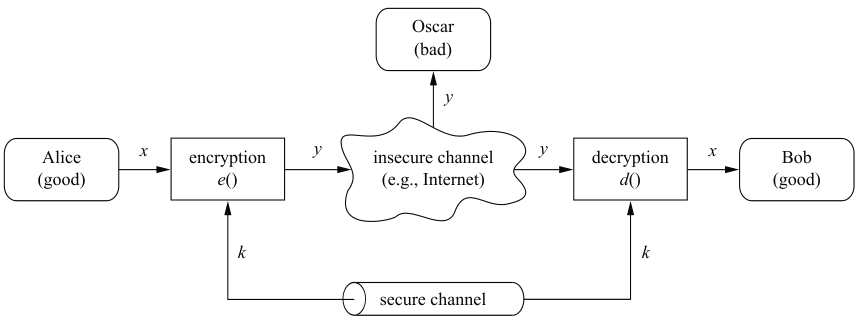
\includegraphics[width=.9\linewidth]{img/sym_alg.png}
\caption{Sơ đồ hệ mật mã Khóa Đối xứng}
\label{fig:sym_alg}
\end{figure}

Sơ đồ \ref{fig:sym_alg} minh họa một ứng dụng mật mã Khóa Đối xứng trong thực tế. Alice và Bob là 2 người bạn cần trao đổi thông tin bí mật bằng phương pháp sử dụng mật mã Khóa Đối xứng. Trong khi đó Oscar luôn tìm cách giải mật thông tin nghe được giữa Alice và Bob. Nhưng Alice và Bob có được khóa nên liên lạc được, chỉ Oscar thiếu duy nhất khóa để giải mật nên không thể hiểu thông tin.

Các ký hiệu trong sơ đồ \ref{fig:sym_alg}:
\begin{itemize}
\item x là bản rõ
\item y là bản mật
\item k là khóa 
\end{itemize}

\textbf{Mật mã Khóa Bất đối xứng} dùng hai khóa Cá nhân và khóa Công khai trong thuật toán tạo mật mã và giải mật, cặp khóa có liên hệ chặt chẽ nhau về toán học. Khóa Công khai được công bố cho cộng đồng sử dụng nên dễ bị lộ, còn khóa Cá nhân chỉ có cá nhân được sở hữu. Mặc khác khóa Công khai bị lộ thì cũng rất khó (sử dụng Phân tích mật mã) có thể tìm được khóa Cá nhân.
Khóa cá nhân dùng để tạo mật mã và tạo chữ ký số. Khóa công khai dùng để giải mật mã và xác thực chữ ký số. Ví dụ: khi mật mã dùng một khóa công khai thì chỉ có khóa cá nhân của cặp khóa đó mới giải mã được; Tương tự, dùng một khóa cá nhân tạo chữ ký số thì chỉ có khóa công khai tương ứng mới xác thực chữ ký số đó.

\subsection{Hàm băm}

Hàm băm là phép biến đổi một chiều có đầu vào là thông điệp chiều dài bất kỳ thành một dãy bit có độ dài cố định (tùy thuộc vào thuật toán băm). Giá trị băm còn gọi là hash value (hay Digest) là đặc trưng cho thông điệp ban đầu.

Ví dụ: Với thông điệp ban đầu là Hello world sẽ có các giá trị băm tương ứng với một số hàm băm, như sau:

Adler32: 18ab043d

MD5: 3e25960a79dbc69b674cd4ec67a72c62

SHA-256: 64ec88ca00b268e5ba1a35678a1b5316d212f4f366b2477232\ldots 37f3c

Băm là một giải pháp tạo ra một đặc trưng cho một file dữ liệu. Tương tự như mỗi một con người có một dấu vân tay đặc trưng. Vì vậy Băm còn được gọi dấu vân tay (Fingerprint) của file dữ liệu.

Hàm băm (Hash Function) là một dạng mật mã tạo bản mật không cần giải mật mà đáp ứng yêu cầu kiểm tra tính toàn vẹn của một dữ liệu dựa trên đặc trưng vân tay của nó.

Hàm băm H(x) có khả năng bảo mật tốt, nếu thỏa 3 tính chất: 
Một chiều (One Way),  Tự do liên kết yếu (Weakly Collision Free) và Tự do liên kết mạnh (Strong Collision Free).

\begin{itemize}
\item \emph{Tính chất Một chiều}: Cho trước giá trị băm y, rất khó tìm được x: H(x) = y. Điều này có nghĩa là nhận được giá trị băm y, rất khó tìm được dữ liệu gốc x thỏa: H(x) = y. Tính chất này đảm bảo rất ít tệp dữ liệu có H(x) = y.

\item \emph{Tính chất Tự do liên kết yếu}: cho trước tập dữ liệu x, rất khó tìm được tệp dữ liệu x’≠x: H(x)=H(x’). Nếu x là tập dữ liệu cần băm, thì hầu như không thể tìm được tập dữ liệu khác x’: H(x’)=H(x). Tính chất này đảm bảo tệp dữ liệu x kèm H(x) rất khó bị sửa thành x’ có cùng H(x).

\item \emph{Tính chất Tự do liên kết mạnh}: rất khó có thể tìm được 2 tập dữ liệu x ≠ x’ có cùng giá trị băm H(x) = H(x’).
\end{itemize}






\subsection{Chữ ký số}
Chữ ký số được định nghĩa là một loại chữ ký điện tử, được tạo bằng sự chuyển đổi thông điệp dữ liệu sử dụng một hệ thống mật mã không đối xứng, theo đó người có được thông điệp dữ liệu ban đầu và khóa công khai của người ký có thể xác định được chính xác.

\begin{enumerate}[a)]
\item Việc biến đổi nêu trên được tạo ra bằng đúng khóa bí mật tương ứng với khóa công khai trong cùng một cặp khóa;
\item Sự toàn vẹn nội dung của thông điệp dữ liệu kể từ khi thực hiện việc biến đổi nêu trên.
\end{enumerate}

Chữ ký số có chung mục tiêu như chữ ký tay trên văn bản. Đó là cách xác định một người bằng dấu vết riêng tác động lên văn bản và qua đó văn bản được ký là chứng cứ sự thật do người đó tạo lập nên. Chữ ký số là thành phần quan trọng trong những giải pháp ứng dụng mật mã, và được áp dụng rộng rãi trong thực tiễn cho đến nay. Chữ ký số cùng với cơ chế trao đổi khóa là cơ sở quan trọng trong hạ tầng khóa công khai. Tuy nhiên, chữ ký số chỉ có thể đảm bảo khi khóa bí mật không bị lộ. Khi khóa bí mật bị lộ thì người sở hữu chữ ký không thể ngăn chặn được việc bị giả mạo chữ ký.

\subsubsection{Nguyên lý ký số và xác thực chữ ký số }

\begin{figure}[htbp]
\centering
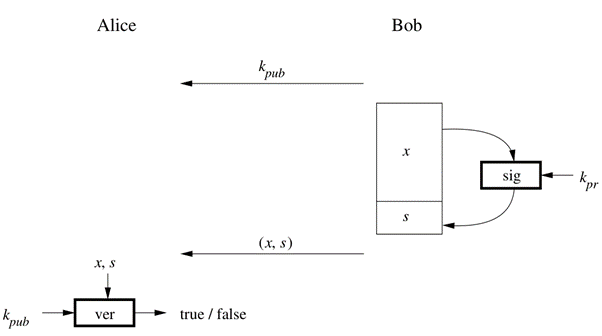
\includegraphics[width=.9\linewidth]{img/dig_sig.png}
\caption{Sơ đồ ký số và xác thực chữ ký số thông điệp}
\label{fig:dig_sig}
\end{figure}

Quy trình bắt đầu khi Bob ký thông điệp x. Thuật toán ký số (sig) có tham số thứ nhất là khóa bí mật của Bob, $k_{pr}$ . Khóa bí mật được Bob giữ và chỉ anh ta mới có thể ký số lên thông điệp x. Thông điệp x là tham số thứ hai của thuật toán ký số. Sau đó bản chữ ký s sẽ thêm vào thông điêp x tạo một cặp (x,s) gửi cho Alice.
 
Tiếp theo Alice xác minh chữ ký của hợp lệ hay không, hàm xác thực (ver) có 2 tham số (x,s) và $k_{pub}$  của Bob. Nếu x do Bob ký số thì được kết quả true, ngược lại false.
Sơ đồ nguyên lý ký số và xác thực chữ ký số được mô tả ở hình ~\ref{fig:dig_sig}

Tuy nhiên, với thông điệp x rất lớn thì ký số sẽ chậm và chiếm dung lượng lớn. Như vậy, thay vì ký số lên thông điệp x, thì có thể ký số lên giá trị băm của x = h(x), giá trị h(x) nhỏ hơn thông điệp x, đồng nghĩa sẽ nhanh hơn. 

\begin{figure}[htbp]
\centering
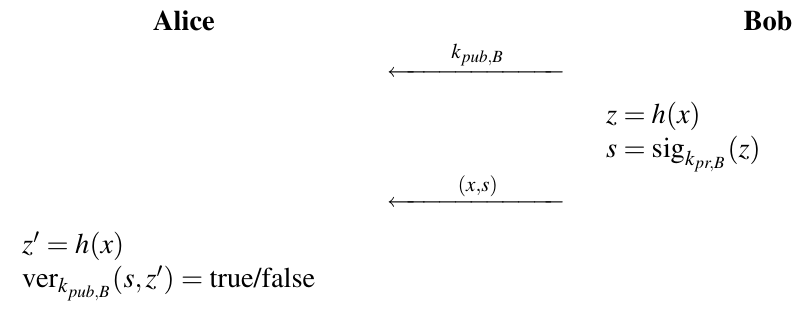
\includegraphics[width=.9\linewidth]{img/dig_sig_hash.png}
\caption{Sơ đồ ký số và xác thực chữ ký số với hàm băm}
\label{fig:dig_sig_hash}
\end{figure}

Bob sẽ tính giá trị băm của thông điệp x và ký số lên giá trị băm z = h(x) bằng khóa bí mật $K_{pr,B}$. Còn bên nhận, Alice sẽ tính giá trị băm z’ của thông điệp x: z’=h(x). Alice sẽ xác thực chữ ký s với khóa công khai $K_{pub,B}$ và z’. Sơ đồ mô tả nguyên lý ký số và xác thực chữ ký số với hàm băm ở hình \ref{fig:dig_sig_hash}

\subsubsection{Chức năng của chữ ký số và tiêu chí an toàn thông tin}
Chữ ký số đảm bảo 2 tiêu chí an toàn thông tin như sau:
\begin{enumerate}
\item Tính toàn vẹn thông tin: khi có sự thay đổi bất kỳ lên thông điệp thì giá trị hàm băm sẽ bị thay đổi; nghĩa là thông điệp không toàn vẹn.
\item Tính không chối bỏ hay chống thoái thác trách nhiệm: vì chỉ có chủ thông điệp mới có khóa bí mật để ký lên thông điệp nên người ký không thể chối bỏ thông điệp của mình
\end{enumerate}

\subsection{Chứng thư số}

Chứng thư số là một dạng chứng thư điện tử do tổ chức cung cấp dịch vụ chứng thực chữ ký số (Certification Authority) cấp nhằm cung cấp thông tin định danh cho khóa công khai của một cơ quan, tổ chức, cá nhân, từ đó xác nhận cơ quan, tổ chức, cá nhân là người ký chữ ký số bằng việc sử dụng khóa bí mật tương ứng. 

Chứng thư X.509 phiên bản 3 có những thông tin sau:
\begin{figure}[htbp]
\centering
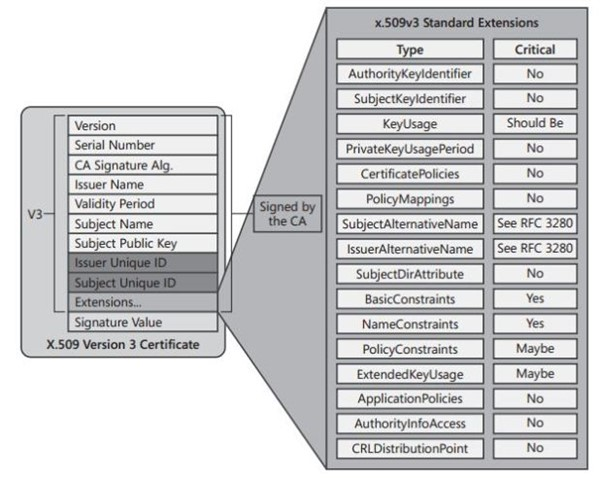
\includegraphics[width=.9\linewidth]{img/x509v3.jpg}
\caption{Cấu trúc chứng thư số X.509 phiên bản 3}
\end{figure}
\begin{itemize}

\item Chủ thể (subject) của chứng thư: thông tin về người dùng, máy tính, thiết bị mạng giữ khóa bí mật tương ứng với chứng thư được cấp phát.
\item Tên dịch vụ chứng thực chữ ký số: thông tin về tổ chức cung cấp chứng thư.
\item Khóa công khai tương ứng với khóa bí mật được liên kết với chứng thư.
\item Tên của các thuật toán để mã hóa và thuật toán tạo chữ ký số cho chứng thư.
\item Trạng thái thu hồi (revocation) và tính hiệu lực của chứng thư (như ngày phát hành và ngày hết hạn).
\item Các phần mở rộng (extension) cho loại chứng chỉ X.509 version 3.

\end{itemize}


\section{Công nghệ Blockchain}

Công nghệ Blockchain có bản thiết kế đầu tiên vào năm 2008 bởi Satoshi Nakamoto và trở thành thành phần cốt lõi của tiền điện tử Bitcoin \cite{nakamoto2008bitcoin}. Công nghệ này đóng vai trò như một quyển sổ cái ghi lại tất cả giao dịch công khai trên hệ thống máy tính ngang hàng theo phương thức mã hoá các giao dịch. Từ đó, các giao dịch phát sinh mà không cần các tổ chức trung gian, tạo ra giải pháp cho các ứng dụng cần sự minh bạch, tính trách nhiệm, bảo mật cao và giảm thiểu các quy trình thủ tục phức tạp.

Trong những năm gần đây, công nghệ blockchain đang được nghiên cứu và ứng dụng vào nhiều lĩnh vực quan trọng trong giáo dục, dịch vụ công, y tế tại nhiều nước trên thế giới. Công nghệ này là một cơ sở dữ liệu phân cấp lưu trữ dữ liệu trong các khối thông tin được liên kết với nhau bằng mã hóa và mở rộng theo thời gian. Mỗi khối được tạo ra đều chứa thông tin thời gian khởi tạo và liên kết với khối trước đó kèm một mã thời gian và thông tin giao dịch. Vì thế, blockchain được thiết kế để chống lại sự thay đổi của dữ liệu. Khi dữ liệu đã lưu trữ trên mạng blockchain thì sẽ khó thay đổi được và nếu được cập nhật sẽ được lưu vết dưới dạng nhật ký. Hiện nay, công nghệ này đang thu hút nhiều nghiên cứu để xây dựng các mô hình mạng blockchain cho các quy trình đặc thù trong tài chính, bầu cử, nông nghiệp,\ldots{} ngoài lĩnh vực tiên phong là tiền mã hóa.

Hệ thống mạng blockchain có thể được chia làm 3 nhóm. (1) Nhóm hệ thống blockchain công cộng cho phép mọi người dùng có thể truy cập dữ liệu như Bitcoin, Ethereum,\ldots{}. (2) Nhóm hệ thống blockchain riêng tư do một tổ chức hoặc một cá nhân đầu tư và kiểm soát, thông tin được kiểm soát chặt chẽ và chỉ được phổ biến trong nội bộ. (3) Nhóm còn lại là hệ thống blockchain cộng đồng là hiệp hội các tổ chức có thể xây dựng riêng mạng cho các thành viên của mình theo nguyên lý blockchain, cơ chế đồng thuận trong cộng đồng phát triển theo xu hướng tin cậy theo đa số trong cộng đồng. Mỗi hệ thống blockchain có những đặc điểm riêng và được ứng dụng trong từng lĩnh vực cụ thể. Trong thực tế, công nghệ blockchain chỉ phù hợp với các dạng dữ liệu giao dịch.

\section{Hyperledger Fabric}

\subsection{Giới thiệu}

Hyperledger Fabric là một trong năm framework về blockchain nằm trong chiến lược Hyperledger Umbrella của Linux Foundation gồm: Hyperledger Indy, Hyperledger Fabric, Hyperledger Iroha, Hyperledger Sawtooth, Hyperledger Burror.

Hyperledger Fabric là một nền tảng công nghệ mã nguồn mở dưới sự cố vấn của IBM, được thiết kế để sử dụng trong môi trường doanh nghiệp, cung cấp nhiều tính năng nổi trội với các nền tảng blockchain đang tồn tại. Hyperledger Fabric có kiến trúc mô-đun linh hoạt và tối ưu hoá cho nhiều ứng dụng trong các lĩnh vực như: tài chính, bảo hiểm, y tế, chuỗi cung ứng, chính phủ\ldots{} 
\begin{figure}[htbp]
\centering
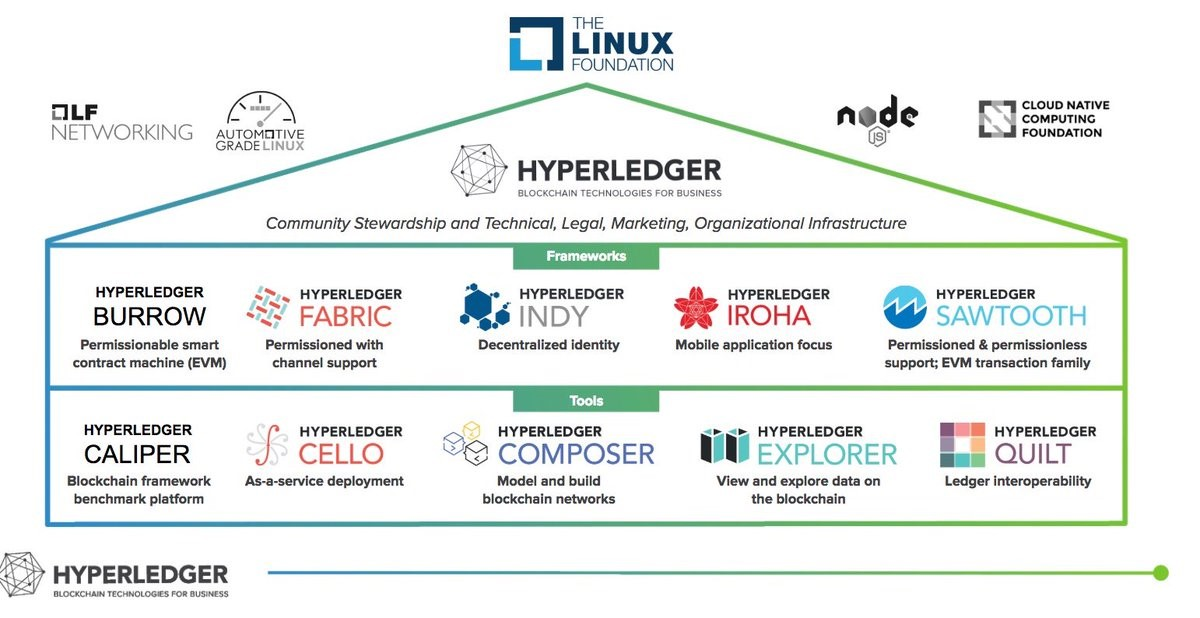
\includegraphics[width=.9\linewidth]{img/hlf_um.jpg}
\caption{Chiến lược Hyperledger Umbrella}
\end{figure}

Nhờ vào thiết kế mô-đun linh hoạt, chính sách quyền hạn cho người tham gia đã giúp Hyperledger Fabric trở thành nền tảng blockchain hoạt động tốt về tốc độ xử lý giao dịch, độ trễ xác nhận giao dịch, cho phép bảo mật và xác minh các giao dịch với hợp đồng thông minh.

\subsection{Những cải tiến của Hyperledger Fabric trong phiên bản 2.x}

Những điểm mới trong phiên bản Hyperledger Fabric 2.x rất thích hợp cho hệ thống mạng blockchain mà đề tài đang hướng đến. Phiên bản mới Fabric 2.x được hỗ trợ dài hạn, điều đó có nghĩa rằng các vấn đề bảo mật, lỗi hệ thống sẽ sớm được công đồng và nhà phát triển cập nhật cho đến khi một phiên bản LTS mới được phát hành.

\begin{figure}[htbp]
\centering
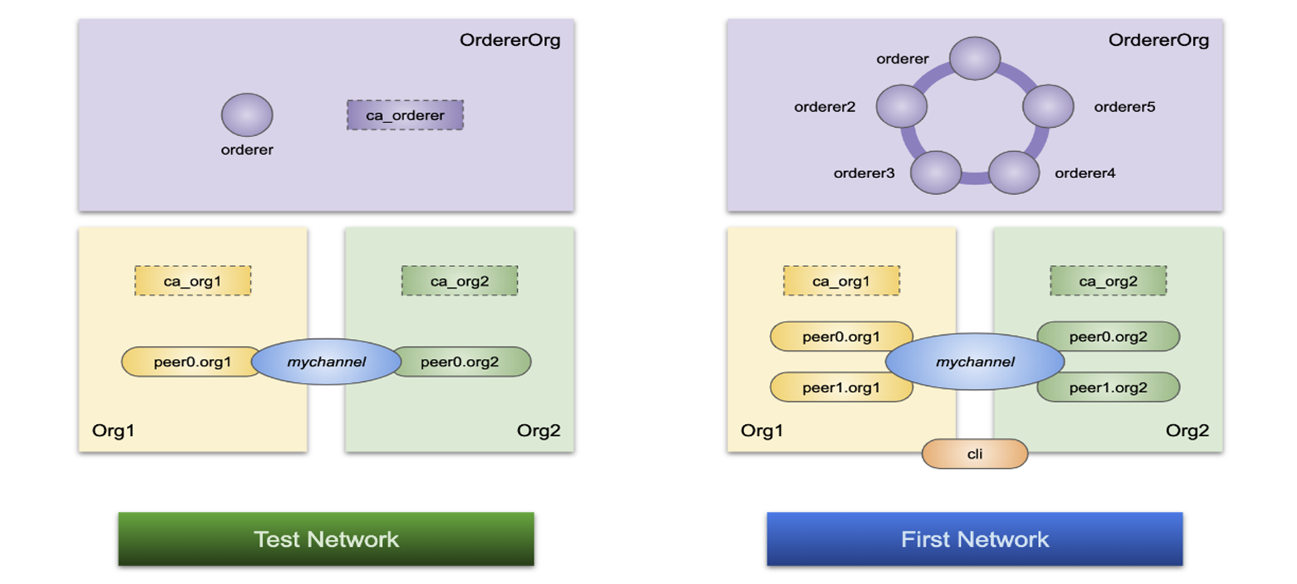
\includegraphics[width=.9\linewidth]{img/hlf_network.png}
\caption{Cấu trúc mạng đề xuất của hai phiên bản 1.4 và 2.x}
\end{figure}

Trong phiên bản Fabric 2.x, các hợp đồng thông minh (chaincode) muốn được cài đặt trên peer và chạy trên channel cần phải thông qua một vòng đời mới. Các tổ chức thuộc kênh (channel) cần thống nhất (đồng ý thỏa thuận) các tham số của hợp đồng như chính sách chứng thực hợp đồng trước khi hợp đồng được thực hiện tương tác với sổ cái (ledger).

Việc nâng cấp các hợp đồng thông minh (chaincode) sẽ được gắn với quá trình đồng thuận và chỉ hoàn thành khi đạt được ngưỡng cho phép của các thành viện thuộc kênh. Điều đó có nghĩa tất cả thành viên thuộc kênh luôn giữ đầy đủ các hợp đồng (được cài đặt chaincode) cùng nhau thay vì có thể từ chối như phiên bản 1.4. Việc thay đổi cơ chế nâng cấp giao dịch của phiên bản 2.x mang lại tính an toàn, đồng nhất dữ liệu so với phiên bản trước.

Dữ liệu riêng tư (Data Privacy) cho phép một phần dữ liệu được chia sẽ riêng tư giữa một số thành viên thuộc kênh thay vì tất cả thành viên đều có thể sở hữu. Thay vì tạo thêm một kênh để nhóm các thành viên và mất rất nhiều thời gian để cấu hình (kênh, chính sách, MSP,…) 

Một trong những điểm nổi bật của phiên bản Fabric 2.x là tối ưu hóa hiệu suất hoạt động của mạng Blockchain. Bằng cách thay thế giải thuật Kafka thành giải thuật Raft, thêm một bộ nhớ đệm mới vào các peer để tìm nạp dữ liệu nhanh hơn khi sử dụng CouchDB bên ngoài, xác thực giao dịch song song, xử lý khối bất động bộ, phân trang chaincode,…Điều đó cho phép Hyperledger Fabric 2.x đảm bảo hiệu suất có thể xử lý hàng nghìn giao dịch mỗi giây. 

\subsection{Các thành phần của mạng Hyperledger Fabric}

\textbf{Ledger}: Một quyển sổ cái bao gồm 2 thành phần có liên quan nhau là “blockchain” và “cơ sở dữ liệu trạng thái”. Các giao dịch thay đổi các tài sản(dữ liệu có cấu trúc) của mạng sẽ được “blockchain” ghi nhận theo dạng nhật ký và không thể xóa hay chỉnh sửa. Ngược lại, “cơ sở dữ liệu trạng thái” (LevelDB hoặc CouchDB) lưu trạng thái mới nhất của các tài sản hiện có trong mạng theo cặp giá trị key-value. Ledgers được lưu trên các Peer trong cùng Channel đồng bộ khi có phát sinh giao dịch thông qua cơ chế đồng thuận.

\textbf{Smart contract} (Chaincode): Hợp đồng thông minh – một ứng dụng được viết bằng các ngôn ngữ lập trình như: Javascript, Go, Java dùng để tương tác với mạng, quản lý tài sản. Trong Hyperledger Fabric, các hợp đồng thông minh được gọi là chaincode, được cài đặt trên các Peer.

\textbf{Peer nodes}: Là thành phần cơ bản của mạng, lưu trữ bản sao của Ledgers và thực thi Smart contract. Các peer được quản lý và duy trì bởi các thành viên trong mạng. Peer được chia làm 2 dạng:

\begin{itemize}
\item \textbf{Endorsing peer}: thực thi các giao dịch trong chaincode và đề xuất giao dịch.
\item \textbf{Committing peer}: có thể không cần cài đặt chaincode, lưu trữ sổ cái đầy đủ.
\end{itemize}

\textbf{Ordering Service (Solo, Raft, Kafka)}: Là thành phần chứa thuật toán đồng thuận và đảm nhận nhiệm vụ xác minh, bảo mật, kiểm định chính sách, quản lý cấu hình Channel.

\textbf{Channel}: Kênh là một “mạng con” riêng kết nối giữa hai hoặc nhiều thành viên trong mạng. Cấu hình một kênh gồm các Orgs(tổ chức), Peer, Ledger, Chaincode, Ordering service. Mỗi Peer có thể tham gia nhiều kênh và sẽ được cấp các định danh riêng với từng kênh bởi nhà cung cấp dịch vụ thành viên (MSP).

\textbf{Fabric Certificate Authorities}: Hyperledger Fabric CA là thành phần phát hành chứng chỉ mặc định, cung cấp chứng chỉ dựa trên PKI cho các tổ chức thành viên mạng và người dùng. CA phát hành một chứng chỉ gốc (rootCert) cho mỗi thành viên và một chứng nhận đăng ký (ECert) cho mỗi người dùng được uỷ quyền.

\textbf{Membership Service Provider (MSP)}: Trong cơ sở hạ tầng của mạng  Hyperledger Fabric, MSP là một tập hợp các thư mục được thêm vào cấu hình của mạng Fabric nhằm xác minh một tổ chức. Đây là một tập hơp các thư mục chứa các chứng chỉ số ( cấp từ CA ), giúp mạng Fabric có thể xác thực các thực thể kết nối với mạng thông qua danh tính (Identities) mà không cần khóa bí mật. Ngoài ra, nó còn có vai trò xác định thực đặc quyền truy cập trong phạm vi mạng và kênh của một thành phần nào đó trong mạng.
%!TEX root = ../luanvan.tex
\chapter{Xây dựng hệ thống}
\section{Tổng quan giải pháp}
Hệ thống quản lý VBCC sử dụng công nghệ blockchain có các chức năng: cấp, quản lý và xác minh VBCC một cách an toàn, bảo mật. Giải pháp được thử nghiệm với nền tảng kỹ thuật số của IBM Blockchain Flatform, Hyperledger Fabric. VBCC có thể được xác thực với tùy chọn hạn chế tiết lộ thông tin và không cần sự can thiệp từ tổ chức cấp chứng chỉ (Trường/Trung tâm).

\begin{figure}[htbp]
\centering
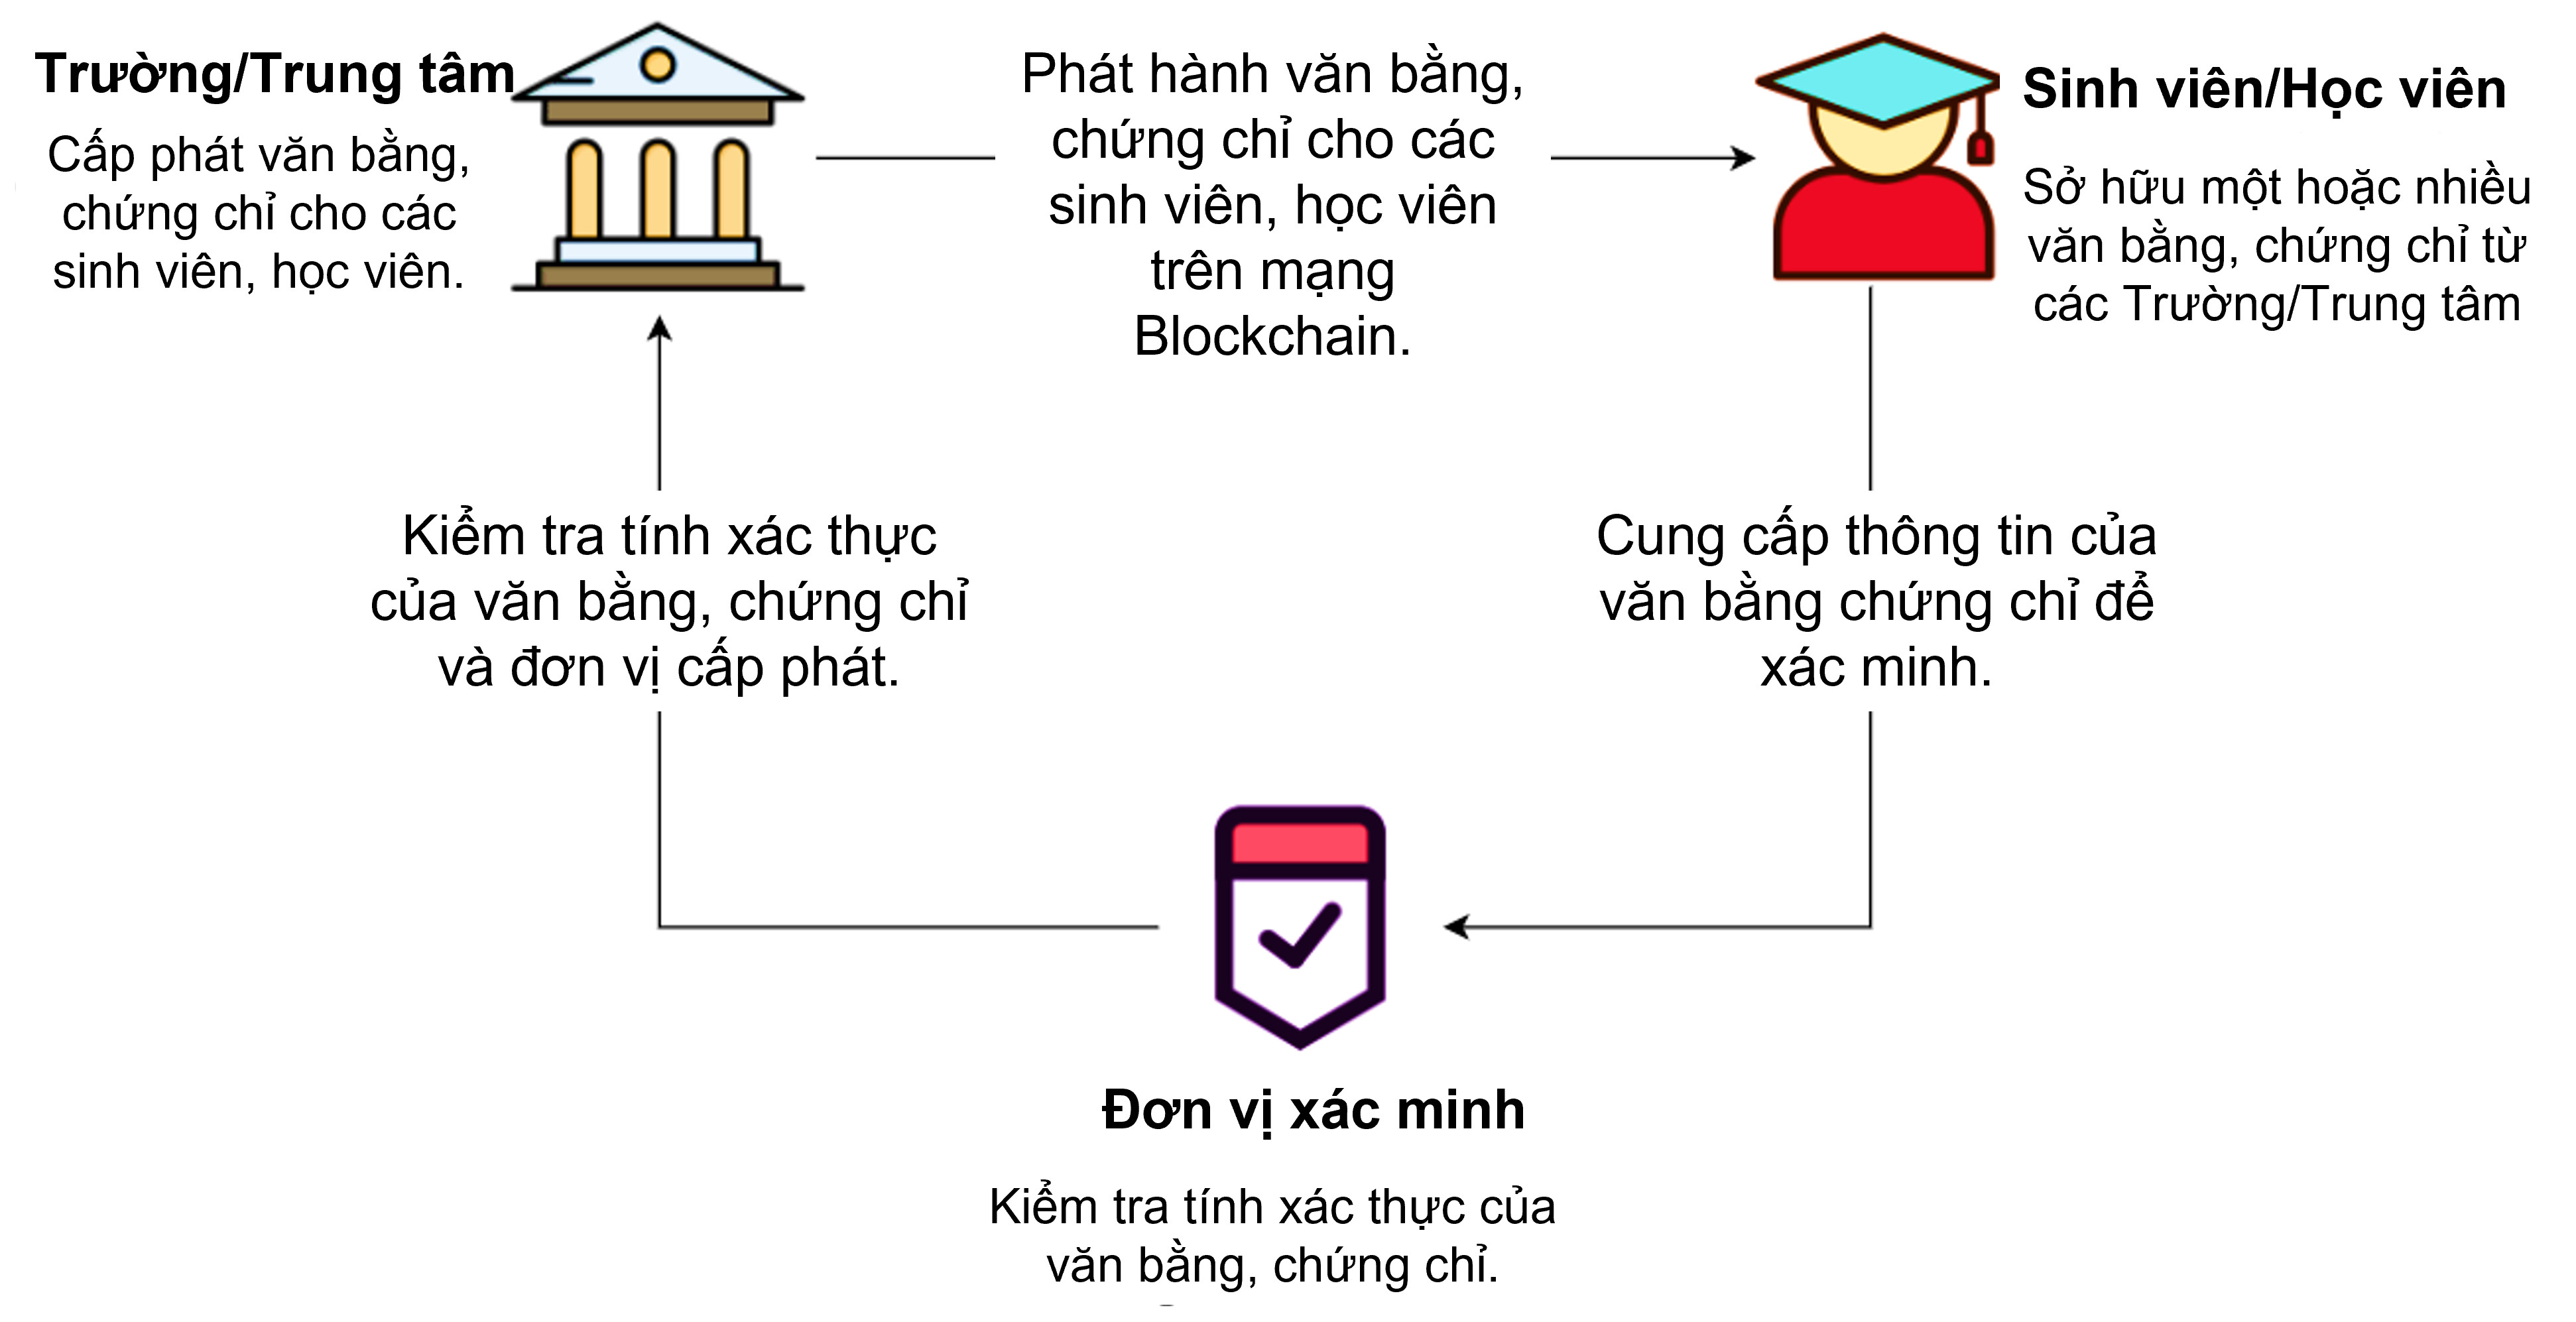
\includegraphics[width=.9\linewidth]{img/vbcc.jpg}
\caption{Sơ đồ tổng quan giải pháp}
\label{fig:vbcc}

\end{figure}
Những chức năng chính của hệ thống được mô tả như hình \ref{fig:vbcc} bao gồm:
\begin{itemize}
\item Trường/Trung tâm: ký số và cấp VBCC.
\item Sinh viên: xem và chia sẻ VBCC.
\item Đơn vị xác minh: kiểm tra tính xác thực của các VBCC được chia sẻ.
\end{itemize}


\section{Kiến trúc phần mềm}
Kiến trúc phần mềm được mô tả như hình \ref{fig:vbcc_phanmem} bao gồm các thành phần:
\begin{figure}[htbp]
\centering
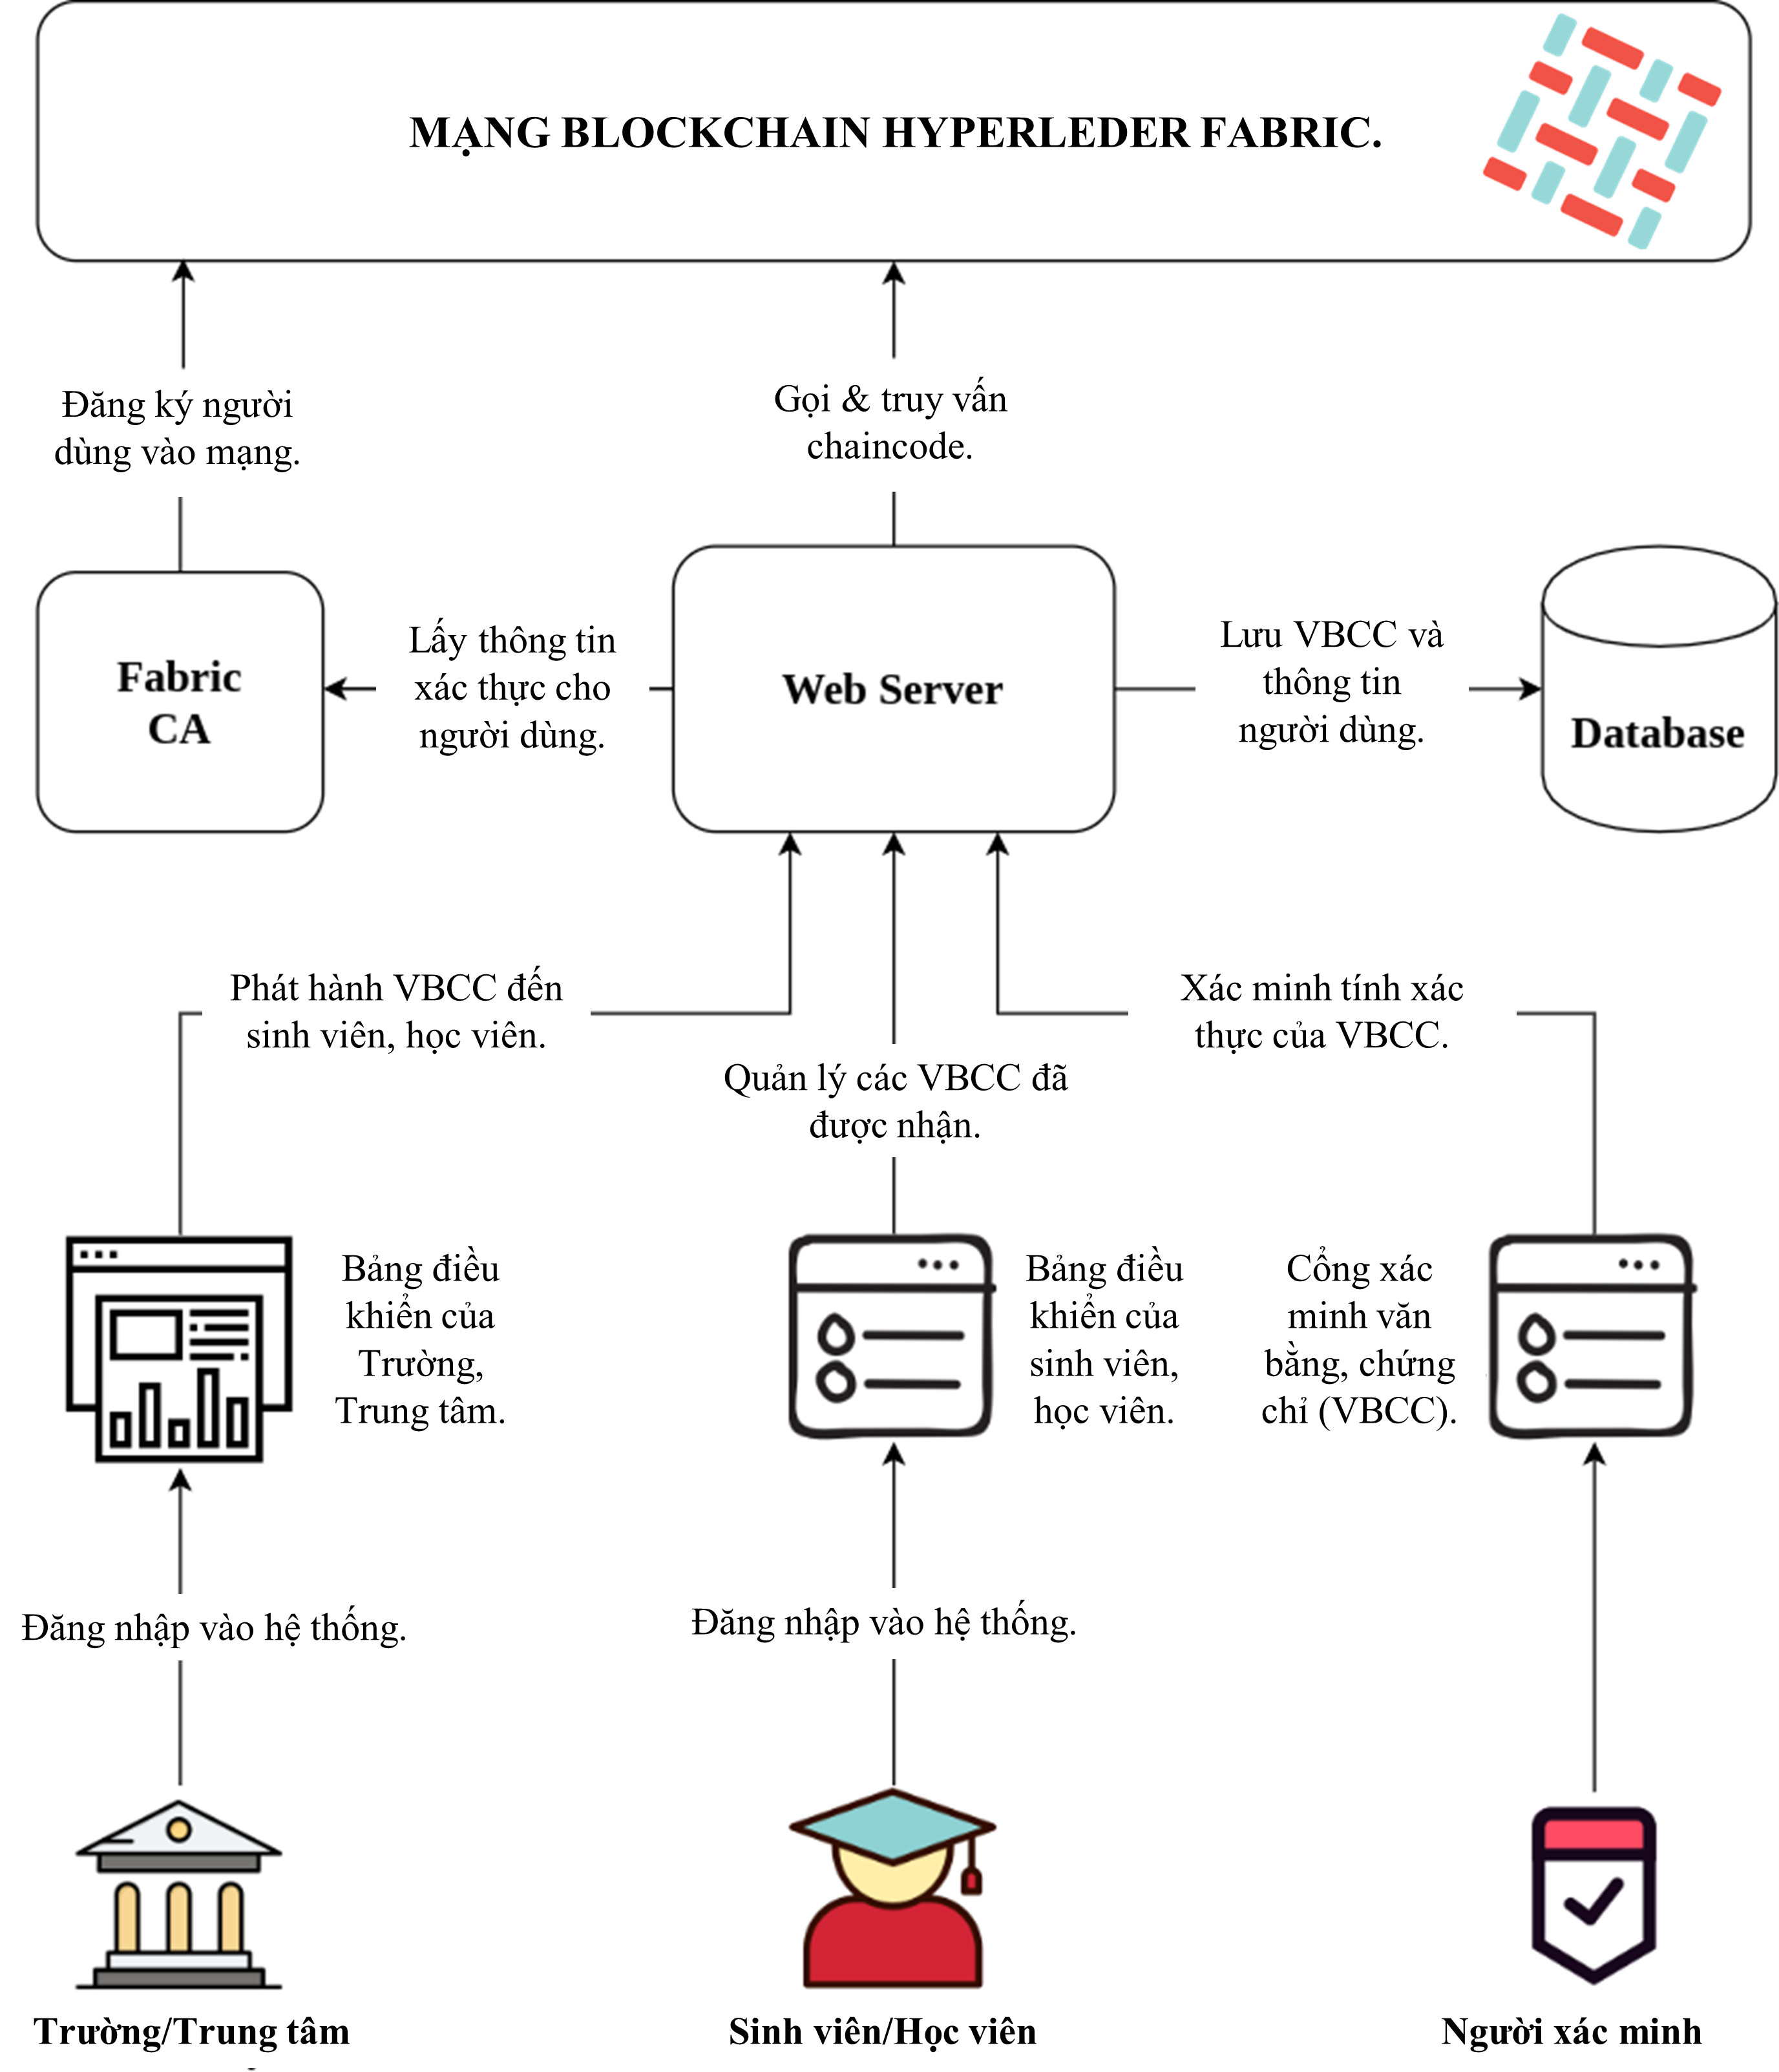
\includegraphics[width=.9\linewidth]{img/vbcc_phanmem.jpg}
\caption{Sơ đồ kiến trúc phần mềm}
\label{fig:vbcc_phanmem}
\end{figure}
\begin{enumerate}
\item Mạng Blockchain Hyperledger Fabric: IBM Blockchain Flatform và Docker container hỗ trợ xây dựng mạng blockchain Fabric, thực thi các hợp đồng thông minh (ngôn ngữ Javascript).
\item Fabric CA: được dùng để đăng ký và xác thực các thành phần trong mạng.
\item Webserver: sử dụng Node.js cung cấp giao diện Backend của ứng dụng web, kết hợp sử dụng Nodejs Express.
\item Cơ sở dữ liệu MongoDB: lưu trữ dữ liệu người dùng và chứng chỉ.
\item Giao diện Front-end của ứng dụng web: dùng các thư viện Bootstrap, jQuery.
\end{enumerate}

\section{Các thành phần tham gia}
Các thành phần tham gia của hệ thống bao gồm: (1) Trường, Trung tâm, (2) Sinh viên (học viên) và (3) Bên xác minh chứng chỉ (Ví dụ: nhà tuyển dụng). Mỗi thành phần sẽ có các hành động như sau:

\emph{Trường, trung tâm}

\begin{itemize}
\item Đăng ký tài khoản.
\item Đăng nhập tài khoản.
\item Cấp VBCC có xác nhận chứng thực và ký số VBCC.
\item Xem VBCC đã cấp.
\end{itemize}

\emph{Sinh viên, học viên}

\begin{itemize}
\item Đăng ký tài khoản.
\item Đăng nhập tài khoản.
\item Xem VBCC đã nhận.
\item Chia sẻ thông tin VBCC.
\item Tiết lộ thông tin VBCC có chọn lọc nhằm hạn chế lộ thông tin.
\end{itemize}

\emph{Bên xác minh chứng chỉ}

\begin{itemize}
\item Xác minh tính xác thực của VBCC với nền tảng blockchain.
\end{itemize}


Quy trình hoạt động của hệ thống được mô tả như hình \ref{fig:vbcc_diagram}

\begin{figure}[htbp]
\centering
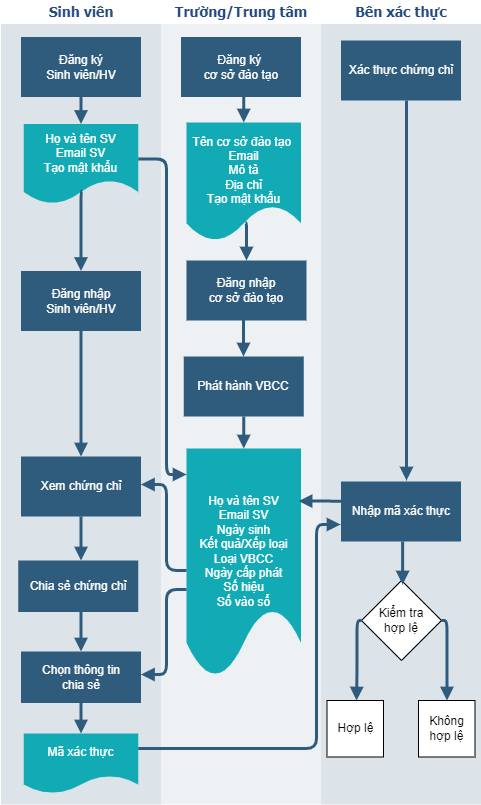
\includegraphics[width=.9\linewidth]{img/vbcc_diagram2.png}
\caption{Quy trình hoạt động của hệ thống}
\label{fig:vbcc_diagram}
\end{figure}

%!TEX root = ../luanvan.tex
\chapter{Kết quả thực nghiệm}
\section{Mạng blockchain}

Mạng Blockchain được cài đặt  trên máy tính cá nhân có cấu hình như sau:
\begin{itemize}
\item CPU: Intel(R) Core(TM) i3-10100F 3.00 GHz
\item RAM: 16 GB
\item Hard Disk: 120 GB NVME SSD
\end{itemize}

Máy tính được thiết lập theo các bước sau:
\begin{enumerate}
\item Mở Visual Studio Code 
\item Tìm extension IBM Blockchain Flatform, chọn cài đặt.
\end{enumerate}
Mạng Blockchain Fabric hoạt động như hình \ref{fig:ide_start}, blockchain thử nghiệm chaincode gồm có tổ chức Org1, peer, CA, Order, OrdererMSP, Org1MSP

\begin{figure}[htbp]
\centering
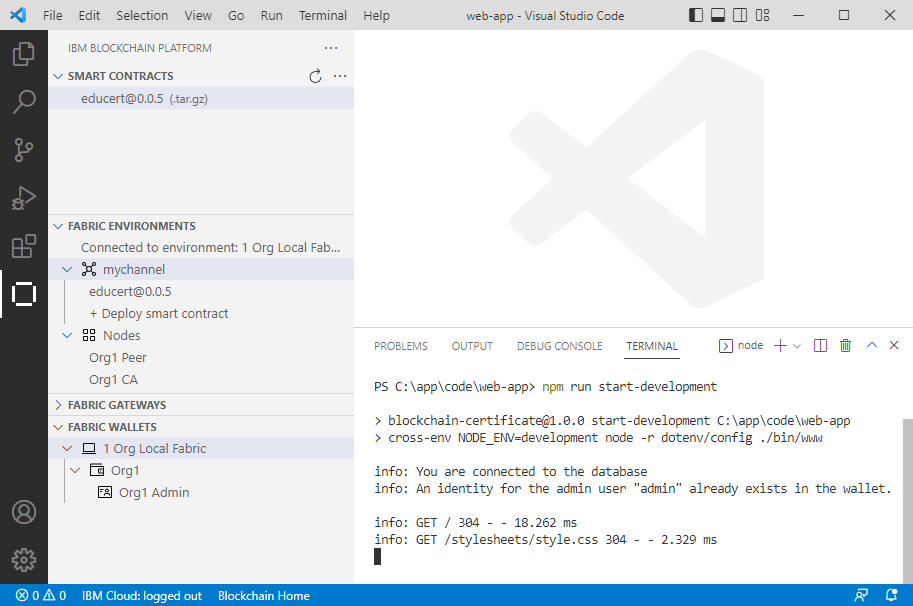
\includegraphics[width=.9\linewidth]{img/ide_start.PNG}
\caption{Chương trình Visual Studio Code}
\label{fig:ide_start}
\end{figure}

\section{Ứng dụng Web}


Giao diện ứng dụng web hoạt động tại địa chỉ http://localhost:3000/ như hình \ref{fig:main_vbcc}. 

\begin{figure}[H]
\centering
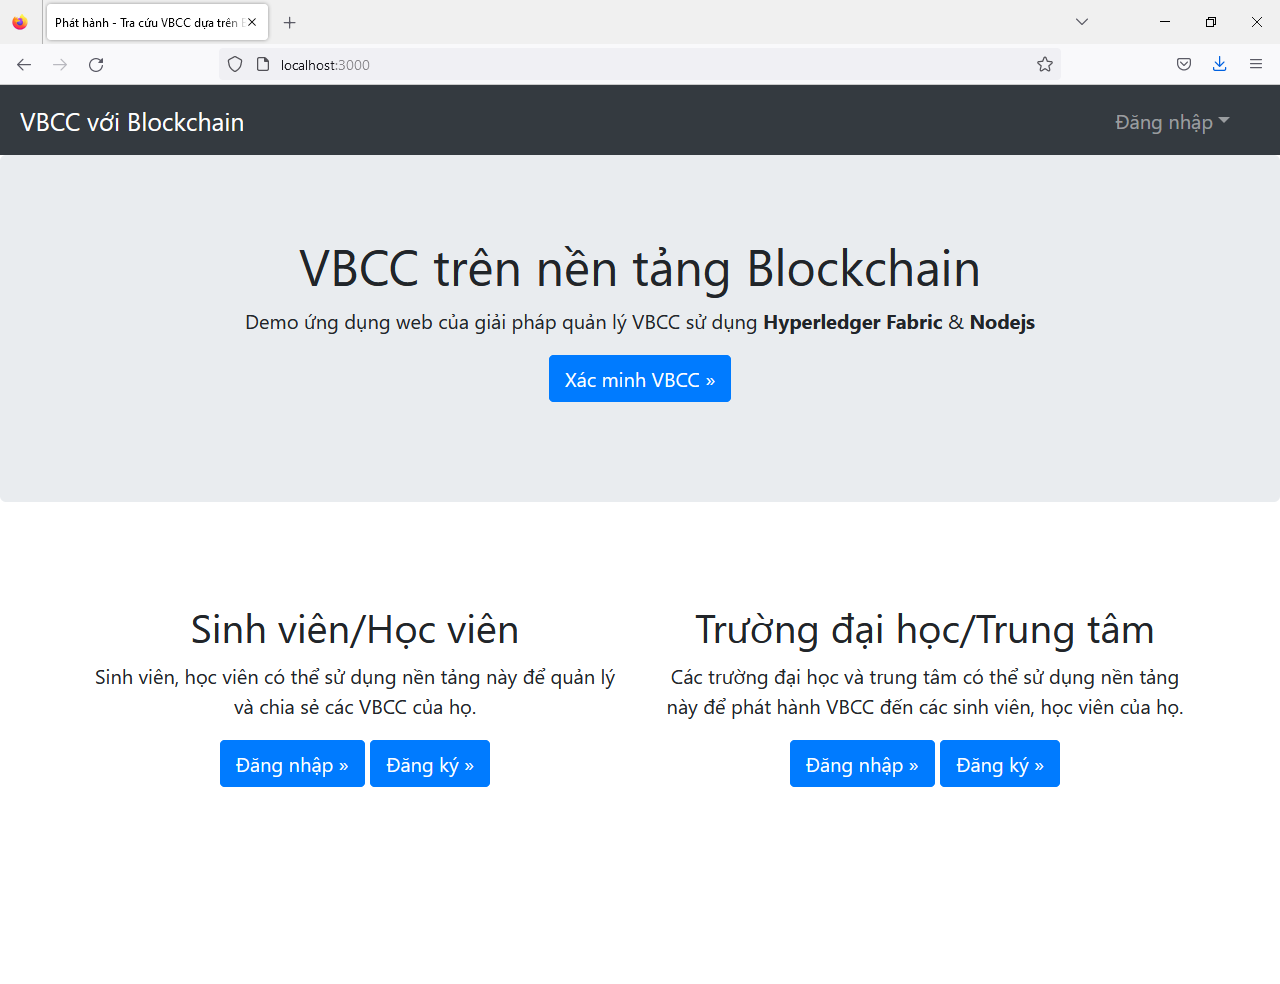
\includegraphics[width=.9\linewidth]{img/main_vbcc.png}
\caption{Giao diện hệ thống}
\label{fig:main_vbcc}
\end{figure}

\textbf{Màn hình chức năng quản lý VBCC của Trường, trung tâm}

\emph{Màn hình phát VBCC cho sinh viên}, hình \ref{fig:tt_phathanh}

Trường thực hiện đăng nhập sử dụng hệ thống. Sau đó, chọn chức năng phát VBCC. 

Sau đó nhập tất cả thông tin VBCC cần thiết để cấp VBCC, trong đó Email của Sinh viên được dùng để tạo mật mã VBCC.
\begin{figure}[H]
\centering
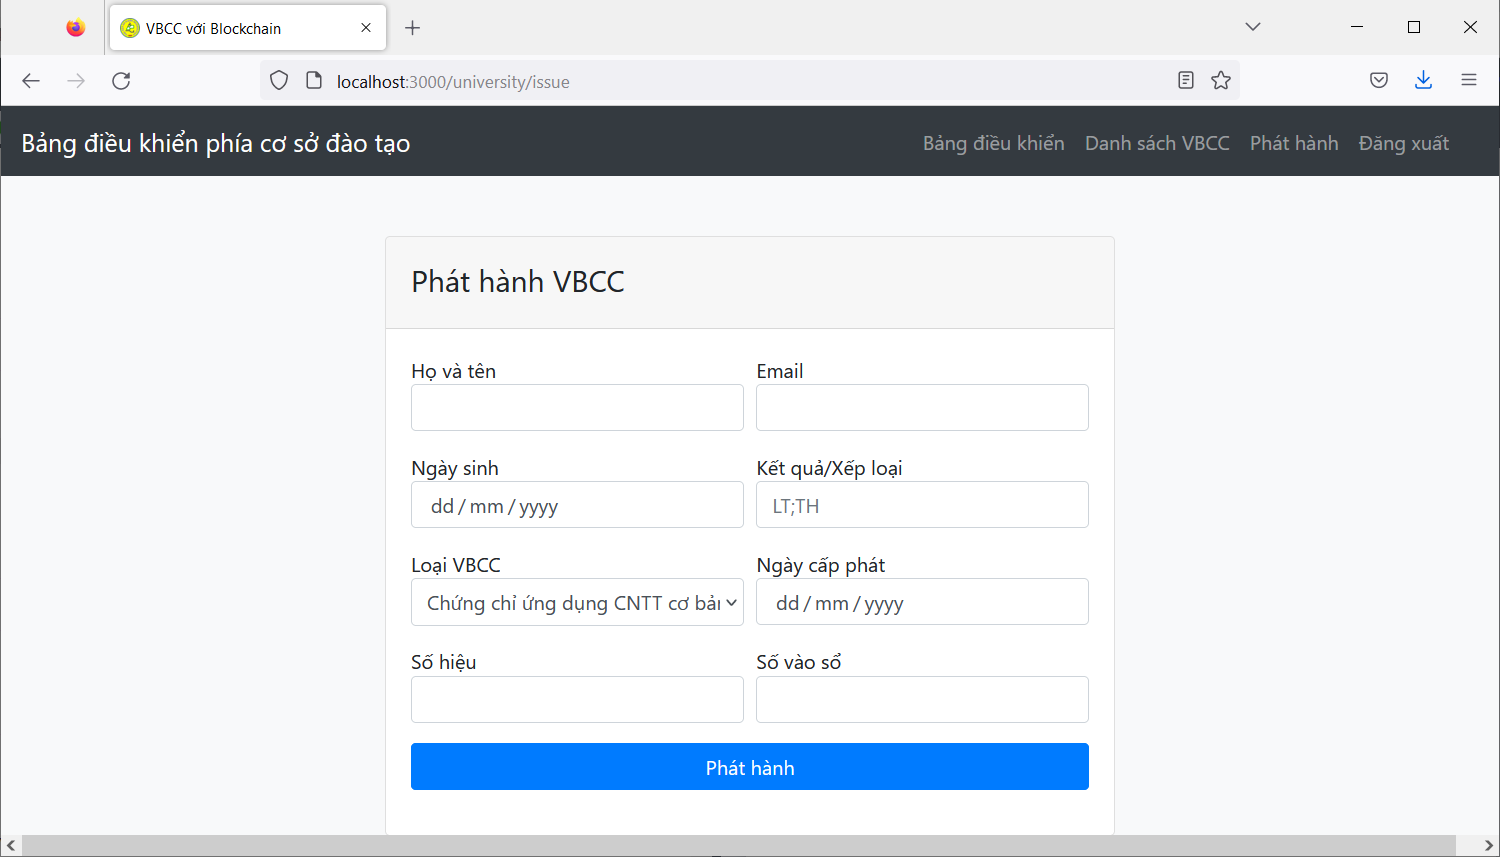
\includegraphics[width=.9\linewidth]{img/tt_phathanh.PNG}
\caption{Màn hình cấp VBCC cho sinh viên}
\label{fig:tt_phathanh}
\end{figure}

\emph{Màn hình xem các VBCC đã cấp cho sinh viên}  yêu cầu Trường thực hiện đăng nhập sử dụng hệ thống. Sau đó,  chọn chức năng xem VBCC. 

\begin{figure}[H]
\centering
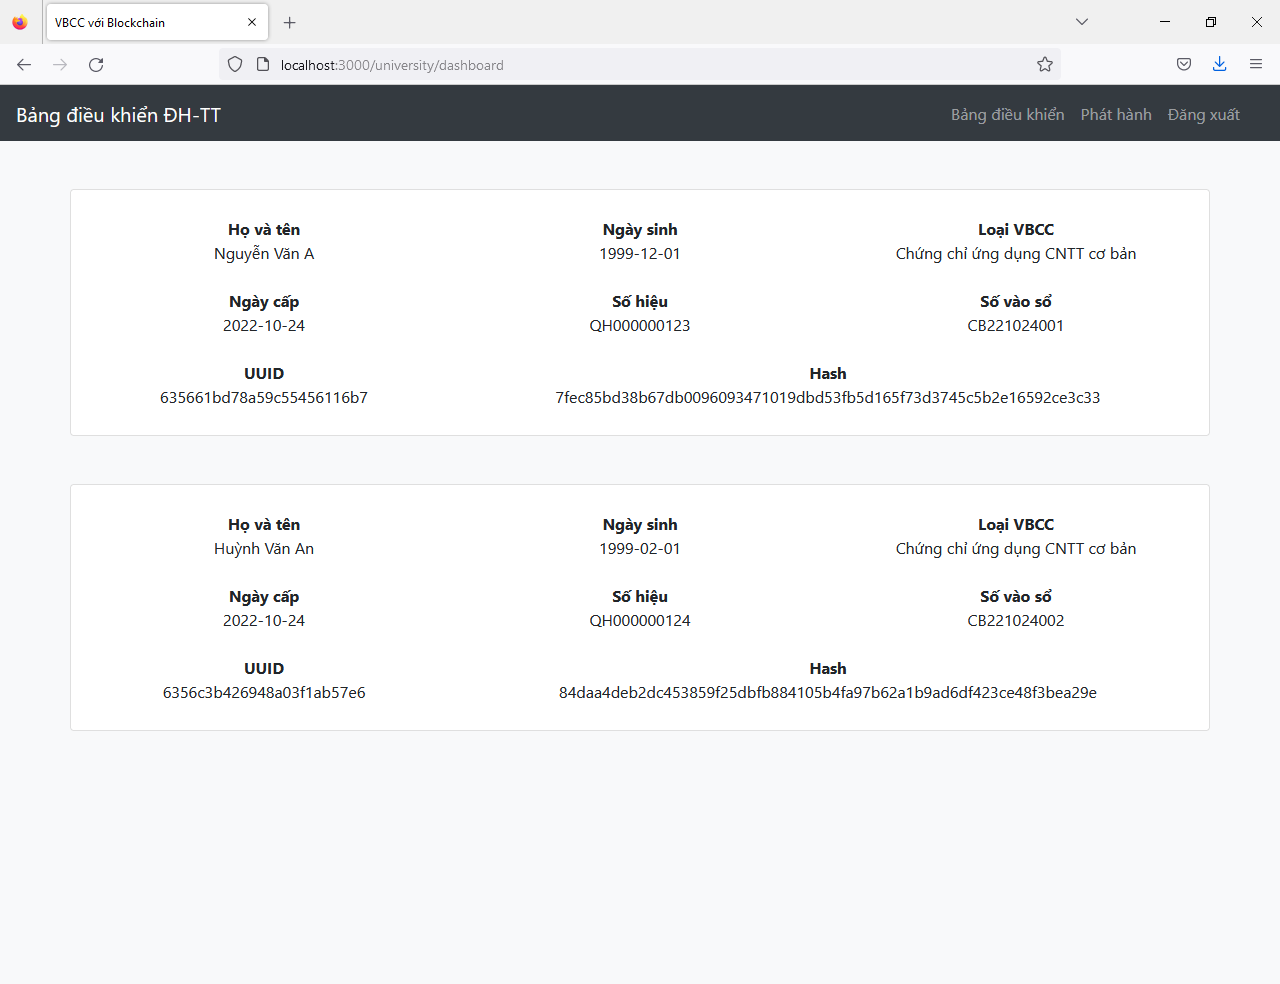
\includegraphics[width=.9\linewidth]{img/tt_dacap.PNG}
\caption{Màn hình xem các VBCC đã cấp}
\label{fig:tt_dacap}
\end{figure}


Sinh viên, học viên có chức năng

Màn hình đăng ký tài khoản.
Sinh viên cần đăng ký tải khoản để sử dụng hệ thống.
Sinh viên nhập thông tin đăng ký, trong đó Email sinh viên dùng để mật mã VBCC.

\begin{figure}[H]
\centering
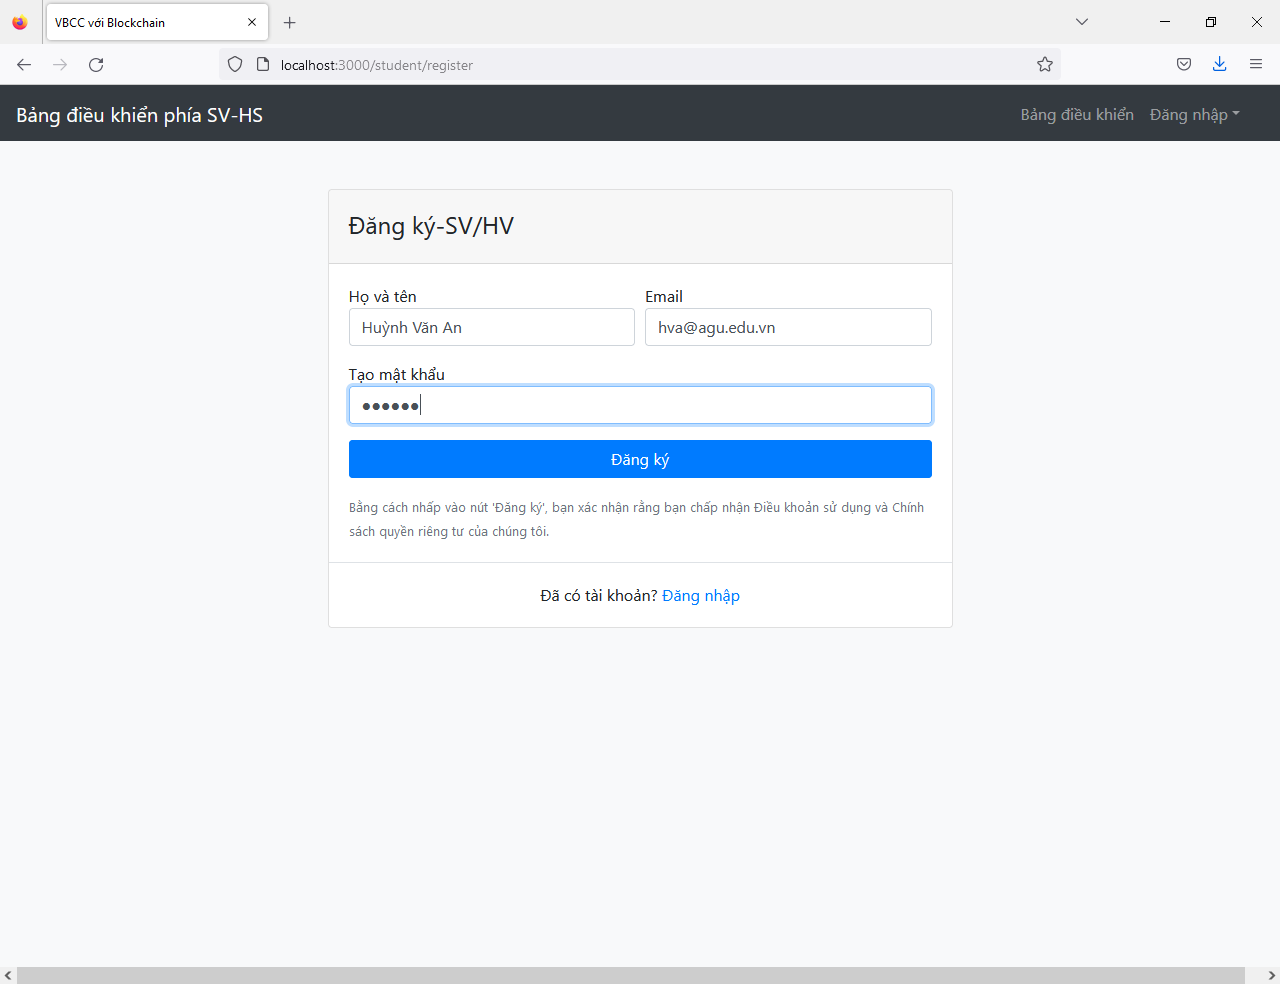
\includegraphics[width=.9\linewidth]{img/std_new.PNG}
\caption{Màn hình đăng ký tài khoản}
\label{fig:std_new}
\end{figure}

Màn hình xem các VBCC đã nhận.
Sinh viên cần đăng nhập tải khoản để sử dụng hệ thống.
Sinh viên chọn xem VBCC.
\begin{figure}[H]
\centering
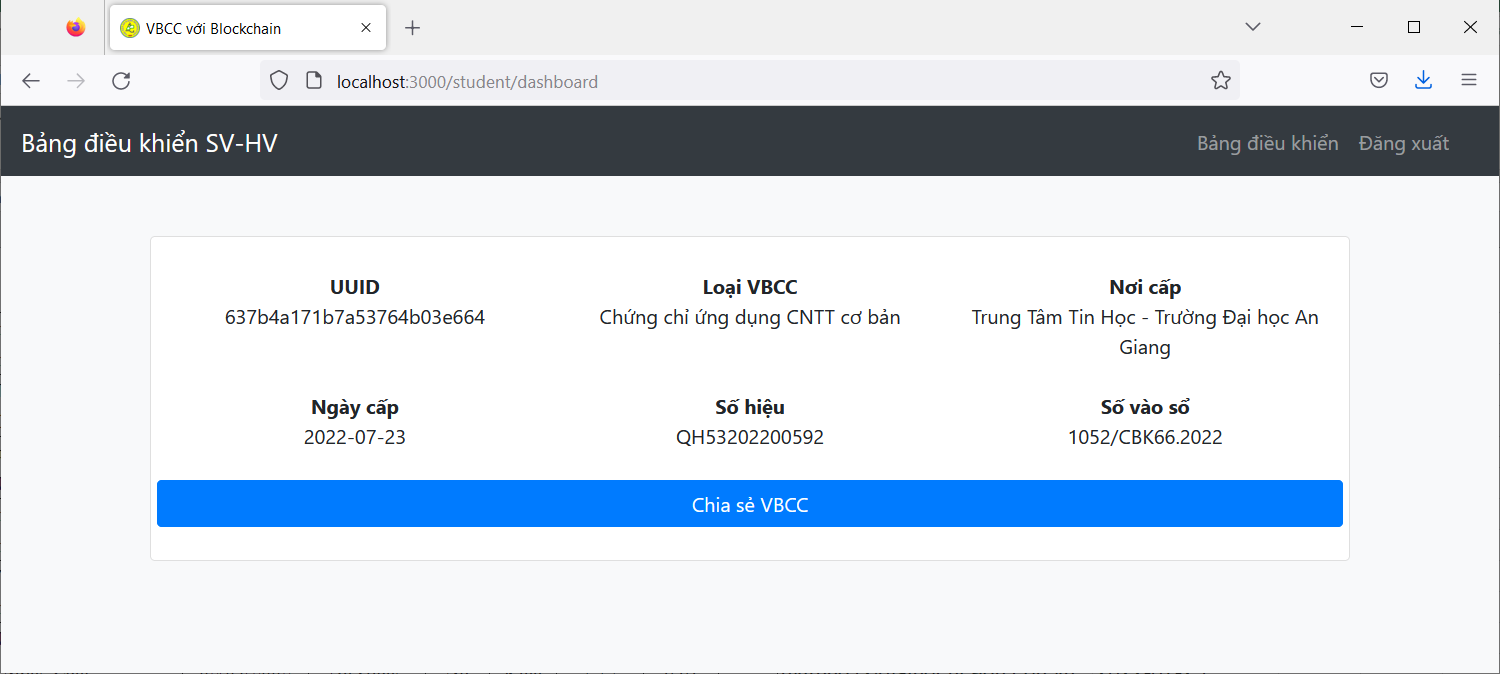
\includegraphics[width=.9\linewidth]{img/sv_hva.PNG}
\caption{Màn hình xem các VBCC đã nhận}
\label{fig:sv_hva}
\end{figure}

Màn hình chia sẻ VBCC đã nhận.
Sinh viên cần đăng nhập tải khoản để sử dụng hệ thống.
Sinh viên chọn chức năng chia sẻ VBCC.
\begin{figure}[H]
\centering
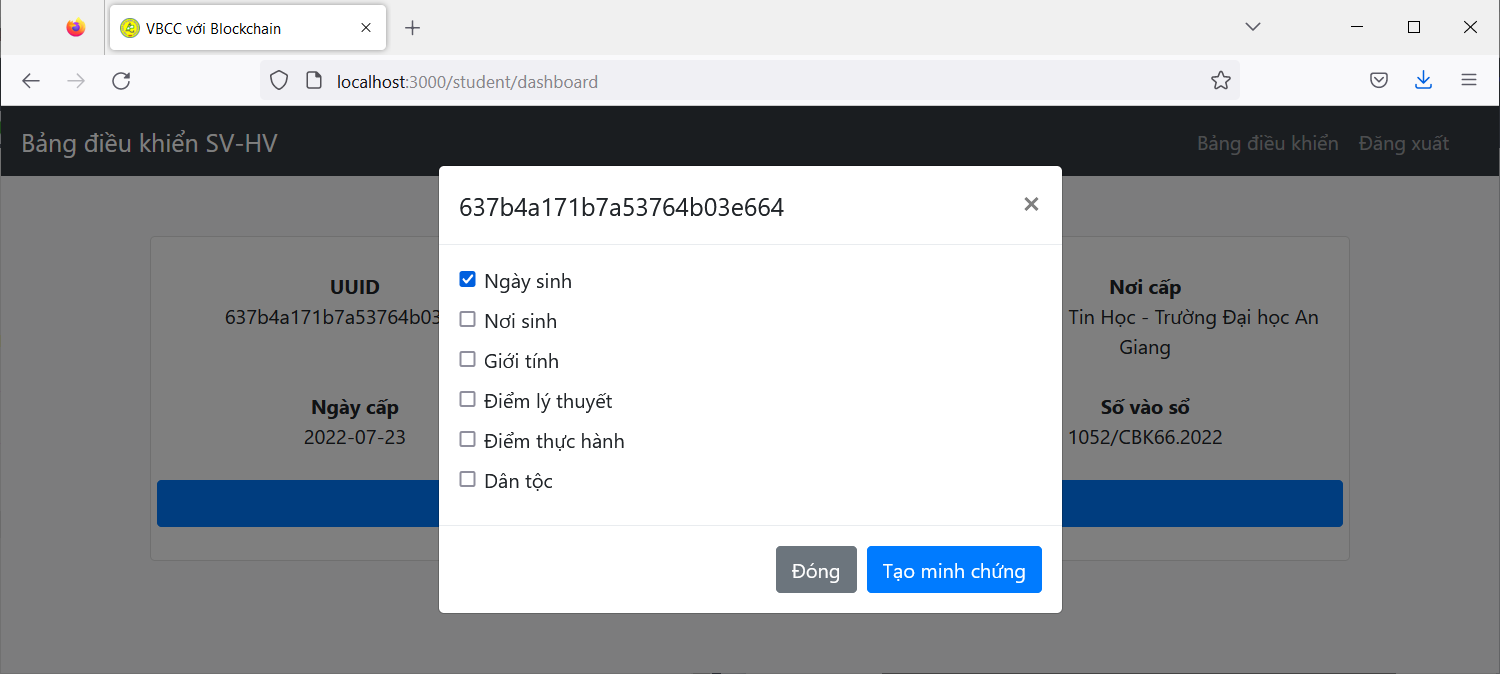
\includegraphics[width=.9\linewidth]{img/sv_chiase.PNG}
\caption{Màn hình chia sẻ thông tin VBCC}
\label{fig:sv_chiase}
\end{figure}

Màn hình chọn thông tin cá nhân chia sẻ.
Sinh viên cần đăng nhập tải khoản để sử dụng hệ thống.
Sinh viên chọn chức năng chia sẻ VBCC.
Sinh viên chọn những thông tin cá nhân cần chia sẻ.
\begin{figure}[H]
\centering
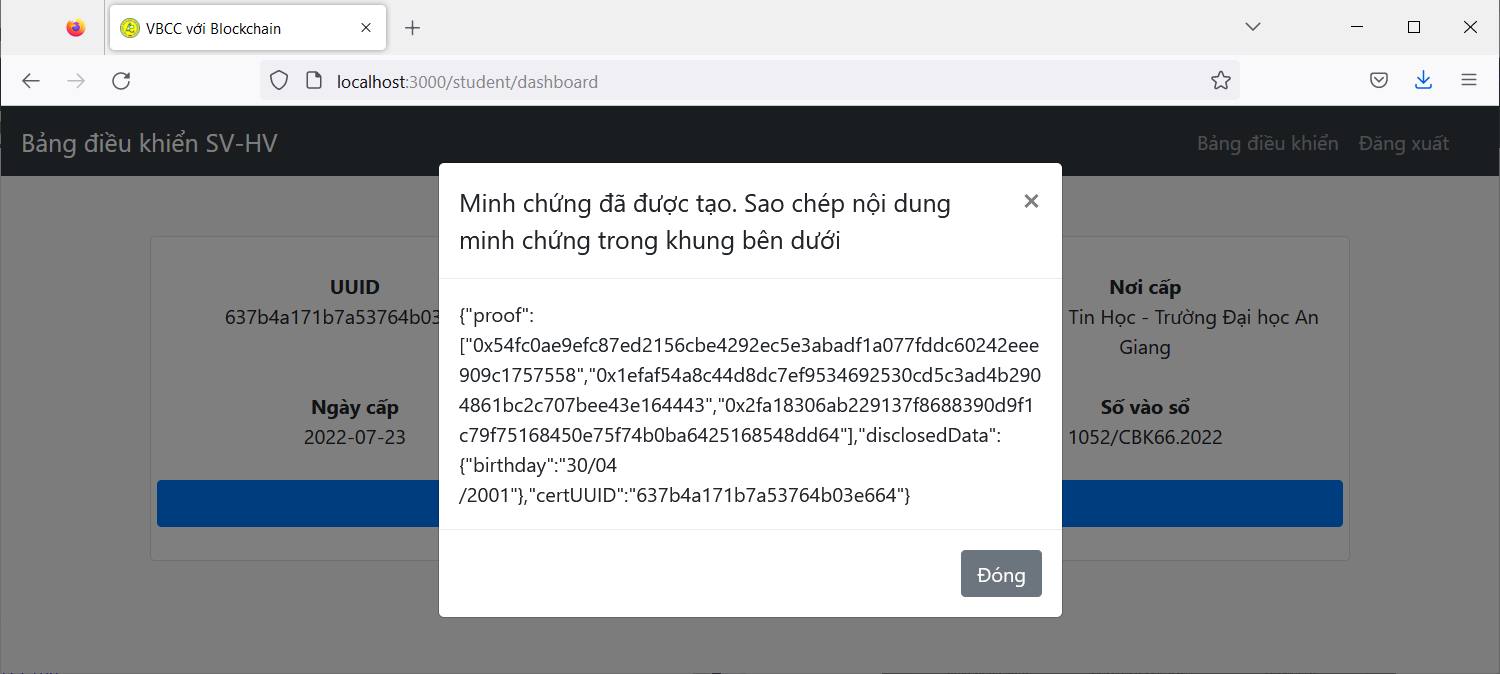
\includegraphics[width=.9\linewidth]{img/sv_minhchung.PNG}
\caption{Màn hình hiển thị mã xác thực VBCC}
\label{fig:sv_minhchung}
\end{figure}

Đơn vị xác minh chứng chỉ có chức năng

\begin{figure}[H]
\centering
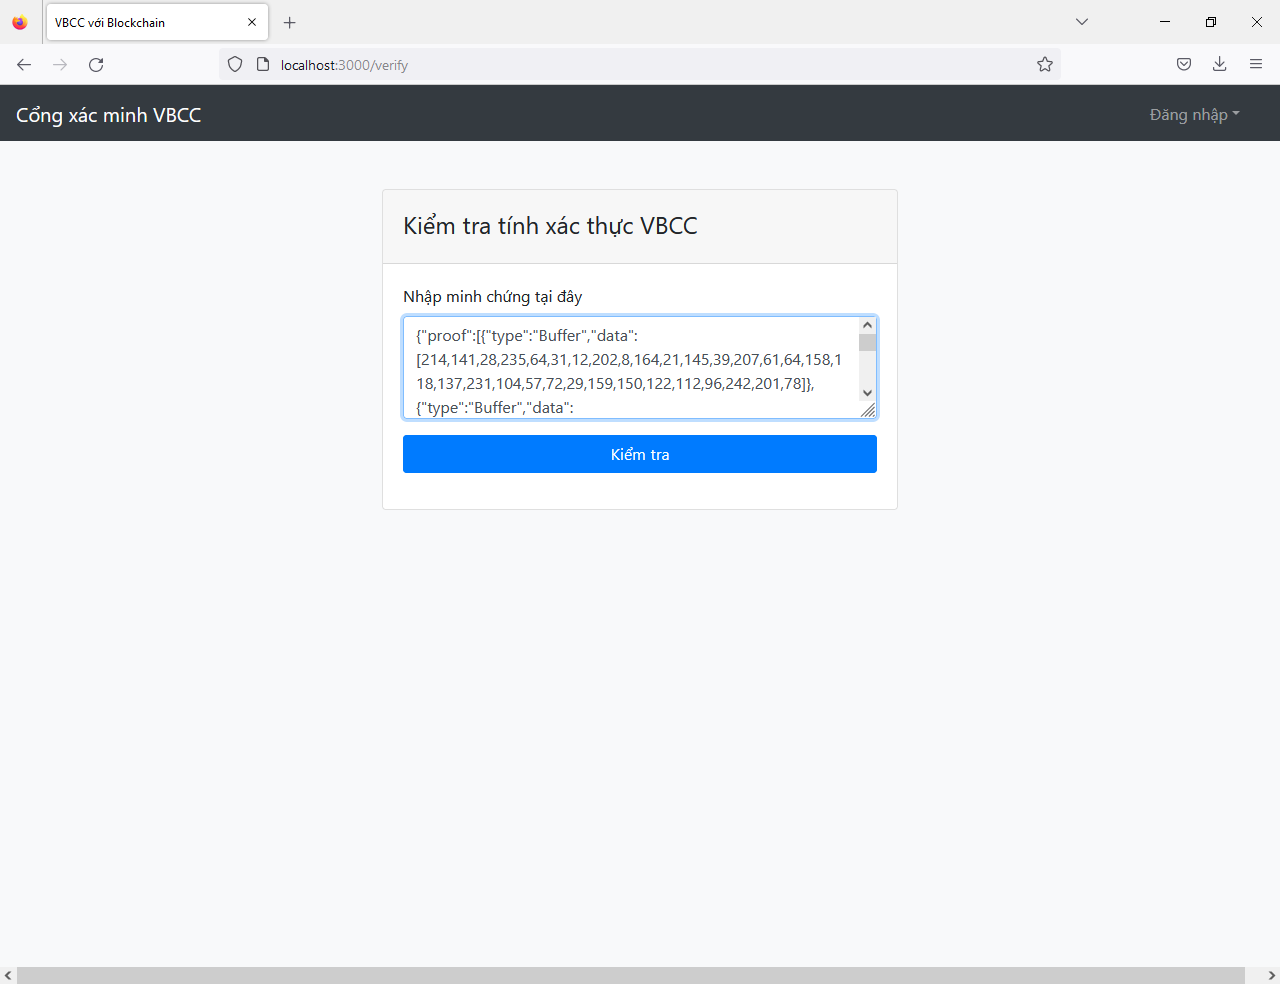
\includegraphics[width=.9\linewidth]{img/v_begin.PNG}
\caption{Màn hình nhập mã xác thực VBCC}
\label{fig:v_begin}
\end{figure}



%!TEX root = ../luanvan.tex
\chapter{Kết luận}
Qua quá trình nghiên cứu, cùng với sự giúp đỡ tận tình của giáo viên hướng dẫn, luận văn đã cơ bản hoàn thành được mục tiêu nghiên cứu, bao gồm một số kết quả sau đây:

\begin{enumerate}

\item Tìm hiểu nghiệp vụ quản lý và văn bản pháp lý về việc quản lý VBCC hiện hành theo quy định của pháp luật và tại Trung tâm Tin học Trường Đại học An Giang; Nghiên cứu tổng quan cơ sở lý thuyết mật mã, công nghệ blockchain và mô hình mạng Hyperledger Fabric.

\item Xây dựng website tương tác với người sử dụng trong việc cấp phát và xác thực chứng chỉ.

\item Xây dựng mạng Hyperledger Fabric để triển khai lưu trữ dữ liệu nhật ký về VBCC trên mạng này.
\end{enumerate}

\textbf{Hạn chế của đề tài}

Hạn chế của đề tài là chỉ dùng dịch vụ chứng thư số của Hyperledger Fabric và chứng thư số tự cấp trong hệ thống. Phạm vi nghiên cứu giới hạn gồm 3 bên tham gia: đơn vị cấp, bên xác minh và sinh viên. Tuy nhiên, cài đặt máy chủ hạ tầng khóa công khai và dịch vụ chứng thư số ở ngoài thực tế là công việc phức tạp và liên quan nhiều vấn đề bảo mật an toàn thông tin cần được quan tâm kỹ lưỡng.

Ngoài ra, dữ liệu nhập vào chuỗi khối đòi hỏi tính chính xác và tin cậy. Do đó đề tài cần tiếp tục nghiên cứu ứng dụng công nghệ blockchain trong quy trình tổ chức thi để có thông tin chính xác từ ban đầu đến khi cấp chứng chỉ. Thông tin cần được theo dõi khách quan, đảm bảo tin cậy cho người có VBCC, cơ quan quản lý và các tổ chức có liên quan.

\textbf{Định hướng nghiên cứu tiếp theo}

Ngoài những hạn chế trên, chắc chắn đề tài còn có nhiều thiếu sót. Do đó, đề tài sẽ tiếp tục việc nghiên cứu, cải tiến sau: (1) Nghiên cứu các thành phần của Hyperledger Fabric để ứng dụng nhiều tính năng hơn do nền tảng này cung cấp. (2) Nghiên cứu mở rộng các quy trình trong công tác tổ chức thi, liên quan đến cấp chứng chỉ. (3) Cải tiến giao diện người dùng giúp thuận tiện trong quản lý VBCC.


\nocite{*}
\bibliography{tailieuthamkhao.bib}
\bibliographystyle{vietnumeric}

\addcontentsline{toc}{chapter}{Tài liệu tham khảo}

\end{document}
